%%
%%  Department of Electrical, Electronic and Computer Engineering.
%%  EPR400/2 Final Report - Main File.
%%  Copyright (C) 2011-2021 University of Pretoria.
%%

\documentclass{epr400}

%% EDIT: Replace the following with your information.
\eprtitle{EPR400/2 Project Report}
\eprcode{EPR400}
\eprcandidatename{M.B. Hanekom}
\eprstudentnumber{1807432}
\eprdate{November 2021}
\eprsupervisor{Prof. I.K. Craig}
\eprcopynum{Electronic copy}

\begin{document}

%% Generate the required title page.
\maketitlepage

%% --- PART 1 ------------------------------------------------------------

\pagestyle{plain}
\pagenumbering{roman}

\eprsec{Part 1. Preamble}

\vspace*{0.5cm}

%% Import the required preamble pages.
%%
%%  Department of Electrical, Electronic and Computer Engineering.
%%  EPR400/2 Final Report - Preamble.
%%  Copyright (C) 2011-2021 University of Pretoria.
%%

This report describes work that I have done in my final year project, developing a robotic vacuum cleaner to vacuum a room autonomously.
\\[2ex]
\textit{Project proposal and technical documentation} \newline
This main report contains an unaltered copy of the approved Project Proposal (as Part 2 of the report).

Technical documentation appears in Part 4 (Appendix).

All the code that I developed appears as a separate submission on the AMS.
\\[2ex]
\textit{Project history} \newline
This project makes use of the kinetic model and obstacle avoidance algorithm by Yiping et al. \cite{6852853}, the mapping algorithm by Wickramaarachchi et al. \cite{8300385} and the navigation algorithms by Hasan et al. \cite{6850799}. These algorithms have been modified extensively and adapted to the requirements of this project. Where other authors' work has been used, it has been cited appropriately, and the rest of the work reported on here, is entirely my own.
\\[2ex]
\textit{Language editing} \newline
This document has been language edited by a knowledgeable person. By submitting this document in its present form, I declare that this is the written material that I wish to be examined on.

My language editor was \makebox[3in]{\hrulefill}.

\vspace*{0.5cm}

\begin{tabular}{lp{1cm}ll}
\makebox[3in]{\hrulefill}  &  & \makebox[1.5in]{\hrulefill} \\
\textit{Language editor signature}  &  & \textit{Date}
\end{tabular}

\vspace*{0.5cm}

\textit{Declaration}
\\[2ex]
I, \makebox[3in]{\hrulefill} understand what plagiarism is and have carefully studied the plagiarism policy of the University. I hereby declare that all the work described in this report is my own, except where explicitly indicated otherwise. Although I may have discussed the design and investigation with my study leader, fellow students or consulted various books, articles or the Internet, the design/investigative work is my own. I have mastered the design and I have made all the required calculations in my lab book (and/or they are reflected in this report) to authenticate this. I am not presenting a complete solution of someone else.

Wherever I have used information from other sources, I have given credit by proper and complete referencing of the source material so that it can be clearly discerned what is my own work and what was quoted from other sources. I acknowledge that failure to comply with the instructions regarding referencing will be regarded as plagiarism.  If there is any doubt about the authenticity of my work, I am willing to attend an oral ancillary examination/evaluation about the work.

I certify that the Project Proposal appearing as the Introduction section of the report is a verbatim copy of the approved Project Proposal.

\begin{tabular}{lp{1cm}ll}
\makebox[3in]{\hrulefill}  &  & \makebox[1.5in]{\hrulefill} \\
\eprthecandidatename       &  & Date
\end{tabular}

%% End of File.


\newpage

%% Add the Table of Contents.
\tableofcontents
\thispagestyle{empty}
\newpage

%% Import the required abbreviation pages.
%%
%%  Department of Electrical, Electronic and Computer Engineering.
%%  EPR400/2 Final Report - Abbreviations.
%%  Copyright (C) 2011-2021 University of Pretoria.
%%

\section*{LIST OF ABBREVIATIONS}

\begin{tabular}{p{3cm}l}
  \textbf{UGV} &  Unmanned ground vehicle \\
  \textbf{SLAM} &  Simultaneous localization and mapping \\
  \textbf{RRT} & Rapidly-expanding random tree \\
  \textbf{SRT} & Sensor-based random trees \\
  \textbf{GPS} & Global positioning system \\
  \textbf{IMU} & Inertial measurement unit \\
  \textbf{MARG} & Magnetic angular rate gravity \\
  \textbf{AWGN} & Additive white Gaussian noise \\
  \textbf{EKF} & Extended Kalman filter \\
  \textbf{UKF} & Unscented Kalman filter \\
  \textbf{FOV} & Field of view
\end{tabular}

%% End of File.

\newpage

%% --- PART 2 ------------------------------------------------------------

\eprsec{Part 2. Project definition: approved Project Proposal}

This section contains the problem identification in the form of the complete approved Project Proposal, unaltered from the final approved version that appears on the AMS.

\newpage

%% Import the approved project proposal
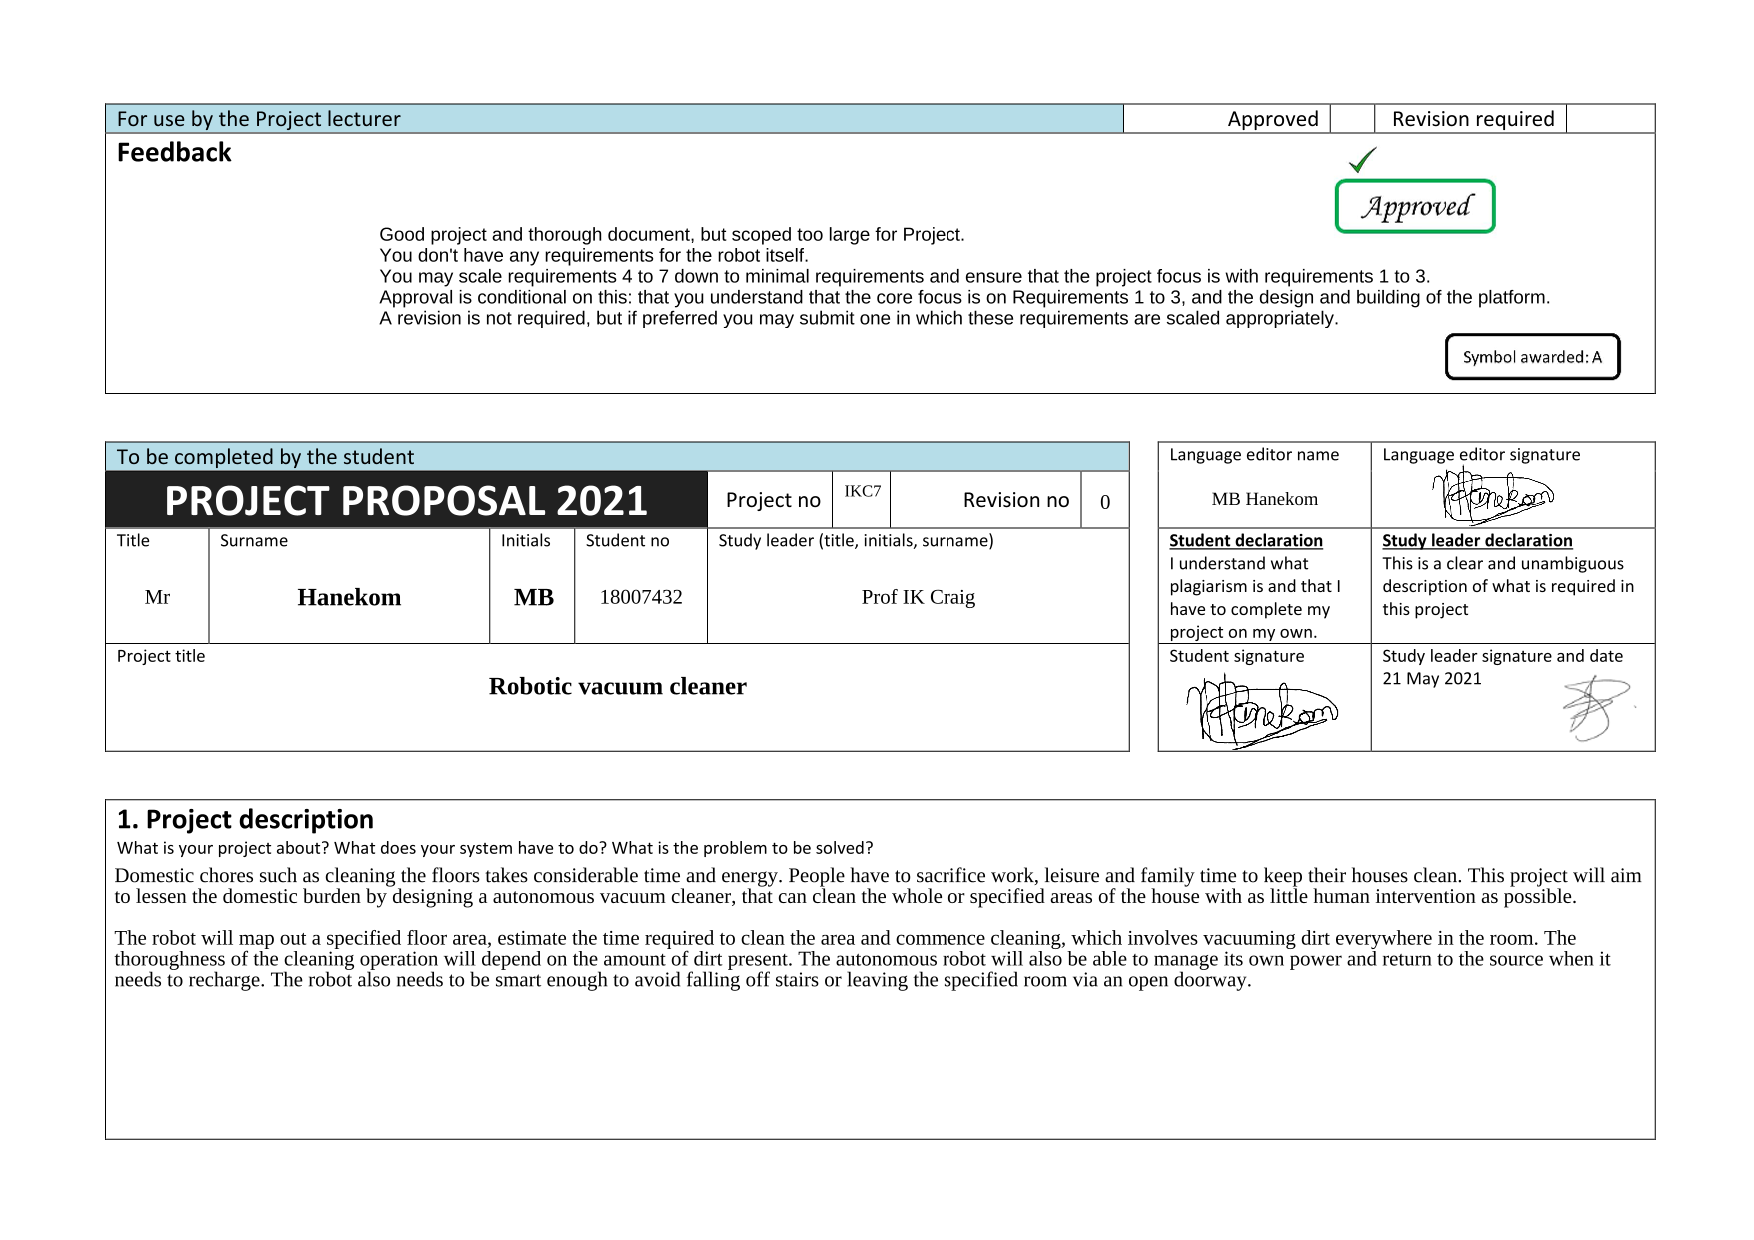
\includepdf[pages=-,landscape]{approved_proposal.pdf}

%% --- PART 3 ------------------------------------------------------------

\eprsec{Part 3. Main Report}
\newpage

%% Reset the page number style and count.
\pagenumbering{arabic}
\setcounter{page}{1}

%% Import the main report content
%%
%%  Department of Electrical, Electronic and Computer Engineering.
%%  EPR400/2 Final Report - Section 1.
%%  Copyright (C) 2011-2021 University of Pretoria.
%%

\section{Literature study}

The world is a vast and mysterious place, full obstacles, dynamic elements and unforeseen circumstances. Robots that have to navigate the world autonomously face a difficult and complex challenge, and require sophisticated solutions to address the uncertainty in sensor data, the danger of the environment and the comprehensive nature of the problem. Autonomous mapping and navigation of a UGV is the cornerstone of mobile robotics. Without a system capable of mapping the world and its location in it, as well as planning paths effectively, a robot relies on human interference
to move around.

\subsection{Positioning and Mapping}

A UGV has to create and maintain an internal representation of the world to navigate around and operate intelligently. The model needs to be at the right level of granularity to interpret the world accurately and efficiently. It consists of a map of the environment as well as an estimation of the robot's position and orientation in it, updated by a process called SLAM. \\

Various SLAM algorithms exists, among which Particle Filter (PF)-SLAM and Graph-SLAM are most prominent. Sugiura and Matsutani \cite{sugiura} investigates the performance of both methods during mapping. PF-SLAM estimates the map and robot position by distributing samples throughout the search space, which are weighted according to the degree of similarity between the sample's estimate of the environment and the sensor's measurement. Larger weights will propagate to the next sample, while smaller ones are removed. Graph-SLAM builds a node-graph while traversing the area, which optimizes the map around closed loops created upon arrival in a previously visited place. \\

An important aspect of both methods is the concept of scan-matching, where local maps built at different timesteps are compared to see if the map and position of the robot can be optimized in such a way that the maps correlate better. Sugiura and Matsutani interpret the map as a grid and evaluate four algorithms: Hill-Climbing, Gauss-Newton, CSM and Branch-and-Bound for optimization. The former two approaches are subject to local maxima, whereas the latter two are computationally expensive. The researchers finally implement CSM, starting with a coarse search map, which iteratively increases in granularity and decreases in size as the proximity of the optimal location is identified. \\

Zooming in on the mapping itself, there are many ways to model the map information obtained from the various sensors measurements, but it is important to choose a model that accurately describes the environment and facilitates quick and easy positioning and navigation. One implementation involves creating a quadtree, as proposed by Han et al. \cite{6393370}, which partitions the known environment into occupied and unoccupied blocks hierarchically, stopping at the coarsest resolution with a uniform occupancy state. This effectively reduces the memory required to store the map and can ease path planning calculations in some applications. \\

An alternative approach involves creating an occupancy map, either bit-wise, where "0" represents open and "1" represents blocked, or probabilistic, where each cell stores the probability that its area is occupied. Chen et al. \cite{9178471} describes a probabilistic occupancy grid map that undergoes optimization via a Bayes Filter.

\subsection{Navigation}

Autonomous navigation is a broad field, and many ingenious algorithms have been developed to address the challenge. The algorithms can be classified into two group according to their goal, in other words the objective that the method is trying to achieve. The first group aims to determine an optimal path to a certain position in a known environment. In essence, these methods try to plan a path to a certain position in the least amount of time and distance covered, without walking into obstacles. The second group of algorithms aim to maximize information gain in an unknown environment, exploring the landscape as efficiently as possible.  \\

A-star search, optimized for navigation in the paper by Ju et al. \cite{9296641}, is the most famous of the first group of path planning algorithms. A-star is a search algorithm with a heuristic, typically provided as the distance to the goal, and a cost, usually the distance travelled to the position, which tries to minimize the sum of the heuristic and the cost at each iteration. The algorithm always chooses the path with the lowest combined heuristic and cost and is thus optimal, even though complete knowledge of the relevant surroundings is needed. The paper adds an improvement to elegantly avoid obstacles similarly to how a human agent would, by heading towards to goal in a straight line while swerving around small obstacles. There is also potential to combine small sequential obstacles to form a larger obstacles that can be navigated more effectively. \\

A path planning algorithm that works on an entirely different principle is RRT. RRT and its improvement RRT*, is described by Chen et al. in \cite{8329210} as a a sampling-based alternative to the slower and more complex algebraic path planning methods. The algorithm randomly chooses the next location in the state space and proceeds in the location's direction by a set or varying amount, exploring new territory and evaluating if the goal has been reached. These class of algorithms are very simple to implement, and can be used in a wide variety of problems, due to the flexibility and generality of the approach. The methods also biases exploration into unknown domains, which helps to rapidly converge on a solution, if one exists. Whereas RRT connect the newly explored node to the geometrically closest node in a tree, the RRT* algorithm seeks to optimize the solution by joining nodes that correspond to the closest distance to that point from the origin. This will produce an optimal result as the number of nodes go to infinity, but suffers from increased complexity and computational burden. \\

The implementation specifically proposed in Chen's paper describes a novel adaptation to the dual tree RRT (DT-RRT), which constructs two trees, one starting at the state and one starting at the goal to simultaneously add nodes in the state space, aiming to converge on a solution sooner. Their paper not only combines dual trees with RRT* rewiring, but also samples in a Gaussian sampling cloud, which is dependent on the state of the system and the context of the problem. They also include methods to deal with boundary problems. This algorithm, being extremely sophisticated, will find use in large and complex path planning problems. \\

The second category of navigation algorithms focuses on exploration and maximizing information gain in the environment. Path planning in an unknown area is inherently more difficult than in known areas, but have seen a lot of research in the past two decades. Groundbreaking work was done by Yamauchi \cite{613851} on frontier-based exploration. He proposes an method that seeks to explore an unknown environment by identifying and moving towards areas of highest potential information gain. This is achieved by constructing an occupancy grid map of the environment, specifying open, unknown and obstructed areas. The frontiers between open and unknown spaces are identified and if a frontier has sufficient size, it will be explored by the robot. The algorithm makes room for dynamic obstacle avoidance in the case that the world changed a bit since the last visit, and will explore all reachable areas in time. \\

Despite the algorithms intuition and completeness appeal, the actual implementation is a lot more daunting. Between the map construction, frontier identification and path planning and obstacle avoidance to potential frontiers, this algorithm has a lot of loosely coupled components, each critical to the success of the operation. Calculating solutions analytically or using search algorithms are exhaustive and potentially burdensome. With this in mind Oriolo et al. \cite{1302457} divised a new method for exploring frontiers, with inspiration from the RRT approach, called Sensor-based Random Tree (SRT). \\

SRT uses the sensor measurements to construct a safe zone around the robot, either as a star, assuming accurate sensor readings in the respective directions, or as a ball, assuming inaccurate measurements and regarding only the closest distance to an obstacle. In either case, a random angle is selected together with a distance in that angle's direction near the edge of the safe zone to obtain a new candidate position node. The position is evaluated to verify that it is far enough away from the current position to justify the move and to make sure it does not fall within an already explored safe zone of a previously explored node. If the candidate fails these checks, a new candidate is chosen until the maximum allows attempts are exceeded, in which case the robot moves back to its parent node. This process ensures that the robot will continuously explore new areas until none are remaining, in which case the robot will return to its original starting position. \\

Combining the random sampling system first seen in RRT with the bias towards frontiers allows the SRT algorithm to implement a simple and effective sampling based exploration mechanism, capable of navigating an unknown environment intuitively with adjustable parameters depending on the sensor specifications of the robot. This makes SRT a simple and extremely flexible navigation tool with a wide range of possible uses and applications.

\subsection{Sensors}

To navigate around and interact with the environment intelligently, a UGV has to perceive the world sufficiently. Various types of sensors exist measuring various aspects of the environment at different accuracies, sample rates and costs. In mobile robotics it is often necessary to obtain information about the environment, such as the location of obstacles, as well as information about the robot itself, such as its measured speed or angular rate. Chan et al. \cite{8616217} recognizes the ubiquity of laser rangefinder in modern UGV systems, which maps the environment as a set of points to the nearest obstacle in a specific direction. The rangefinder is very accurate and its observation data can be used to reconstruct the world map quite effectively. \\

Another common sensor used for obstacle detectior is a monocular camera, first proposed as part of the LSD-SLAM method by Caruso et al. \cite{7353366}. Photos taken by a camera are extremely accurate and full of detail that can be used to reconstruct the environment precisely. The downside is that photos by themselves do not contain depth-information, so a simple analysis of the data do not yield useful results. Instead, the researchers design an intricate system of depth estimation Kalman filters, map optimization and context tracking across frames to analyse the input data. Not only is the process complex, but the photos themselves are large and obnoxious to work with. A laser rangefinder will output an array of distances to the nearest obstacle in the respective directions, totalling a few dozen data points at most. The photos in the paper, on the other hand, has a resolution of 480x480px, accumulating to 230400 data points arriving at 40 Hz. A system would require large computational and memory resources to deal with such a large influx of data. \\

Tracking the robots movement in the environment usually comes down to three sensors: IMUs, GPS and odometers. GPS navigation localizes a user on the ground using positioning data from nearby GPS satellites, and is extremely accurate. However these sensors only work well if there is a clear line of sight between the robot and the satellites, and is generally not suitable for use indoors. \\

IMUs contain a gyroscope, accelerometer in three dimensions, and often comes with a magnetometer as well, then known as a MARG sensor, enabling it to estimation orientation with high accuracy if a suitable filter is used to fuse to sensor data. Harindranath and Arora \cite{8904029} compare four commonly used filters to measure their statistical error and relative performance. Two statistical filters, the Extended Kalman Filter (EKF) and Two stage EKF (TKF-Q), as well as two non-statistical filters, the Mahony and Madgwick filters are compared. The paper aims to analyze the filters in different operating environments, simulating various levels of Gaussian noise, random walk bias and orientation pertubations. While the TKF-Q filter performed well in high levels of noise, the Mahony filters was the winner all around with the lowest average error for static and dynamic simulations with various levels of noise. This filter also benefits from fast execution times. \\

Odometers measure the rotation speed of the wheels attached to the motors, and can be used to determine distance travelled and orientation. Unfortunately wheels can slip, leading to inaccurate measurements, thus in general odometer data is fused with either IMU sensor data or corrected with environment perception optimization. Milijas et al. \cite{9129529} proposes an interactive SLAM-based algorithm, where laser rangefinders are used not only to obtain information of the environment but also to adjust for bad odometry, by viewing both sets of input data in the context of an optimization problem.

\newpage

%% End of File.



%%
%%  Department of Electrical, Electronic and Computer Engineering.
%%  EPR400/2 Final Report - Section 2.
%%  Copyright (C) 2011-2021 University of Pretoria.
%%

\section{Approach}

Designing and constructing an robotic vacuum cleaner capable of autonomous positioning, mapping, exploration and navigation is a rich and complex problem, with many subsystem that need to work together flawlessly for the end product to function. The first important step upon encountering such a large project is to set up a general roadmap and timeline for the design and implementation of the project. The roadmap starts out by evaluating the system requirements and identifies the main problems that the solution needs to address, which are autonomous navigation and floor cleaning in this case. 

These high-level abstract problems are systematically broken down to smaller and more tangible subsystems. Even though the cleaning is a core requirement of the project, it does not entail as much engineering as the navigation, as the project is aimed at computer and not mechanical engineering students, and thus relatively little has to be calculated and designed for the subsystem to function. Autonomous navigation, on the other hand, requires a holistic solution to the problem of robot positioning, mapping and navigation, each with its own sets of challenges and methods, working together in a complex dance. The subsystem's aim is to simultaneously allow the robot to perceive its environment to a sufficient degree that it can interact intelligently with it, and move around in a useful, timely and energy-efficient manner. 

Apart from the software design side, the system has a major hardware component as well. There is a need to identify components and design a layout that contains the necessary sensors, processing power and memory to achieve the goal and to integrate the parts efficiently so that it can be used in a mobile application. There is a bit of a design conundrum here, as the precise implementation of the software is dependent on the hardware components and the hardware requirements is dependent on the software perceived problems. This issue is addressed by identifying the high-level needs of the system software and thereafter searching for available and relevant hardware components (quite a challenge with the global supply chains disrupted). After the first few months of shopping and soldering the first iteration of the robot consisted of an chassis, motors and wheels, a H-bridge and a low-cost processor. 

Next, the basic startup firmware, including timers and peripheral drivers were implemented. The sensor peripherals used to measure distance, angular rate and wheel odometry are adding one-by-one and tested. The use of a Microchip PIC32 chip prohibited the use of standard functions as every single peripheral is initialized manually with register manipulation. This enables the system to run as efficiently as possible, only using exactly what it needs and how it needs it. Optimization of the available real estate on the robot leads to various iterations of the soldered veroboard in this time, with each iteration becoming smaller and using less pins. 

Finally the system is at the point where it can start interacting with the world. Although the software subsystem work together, there is a clear dependency hierarchy, as the mapping depends on accurate real-time positioning and the navigation depends on accurate, real-time mapping. Thus, these subsystems are mostly designed sequentially, iterating back to a previous step once a problem is uncovered. However, before implementation, it was discovered that these systems would be virtually impossible to test objectively using the current evaluation methods. As the reliance on large created data structures and measurement dependent parameters grow, there is no way of knowing why the robot reacts in the way it does without looking into its brain, which would be difficult with a wired serial connection. Instead an OLED screen and Bluetooth serial connection were added to navigate the thought process of the device. 

The positioning subsystem benefits from five sensor measurements: the accelerometer, gyroscope, magnetometer, right and left wheel odometers to update the state of the robot, which includes its position, relative to its internal Cartesian representation of the world. The perceived value and nature of each measurement is evaluated in an elaborate complementary filter. Starting from the systems own estimate of its state given its inputs, which are the PWM duty cycles of the wheels, the estimate is sequentially corrected by the measurements. This approach is favoured due to its simplicity and low computational requirements, whereas the abundance of sensor measurment data aims to bring balance into the equation.

The mapping subsystem faces the challenge of converting the range-based ultrasonic sensor data into an accurate enough representation of the environment so that the robot will not bump into obstacles and clean thoroughly. Three sensors give an idea of the distance to the nearest object in their respective directions, which are offset by $40^\circ$ around the front of the robot. The robot creates a probabilistic map of a certain $cm^2$ resolution to represent the world. Considering that the measurement data contains noise and cannot actually determine the position of an obstacle, just the distance to it in an certain wide field of view, the sequential incoming data is plotted on the probabilistic map as a multivariate Gaussian distribution, with the perceived obstacle positions as the means. Applying a highly efficient multiplication algorithm to the evolving map provides a simple and relatively low cost solution of the perception problem. Of course, there is no use in evaluating parts of the global map that is not currently in range, and thus a smaller local map is updated in the immediate area surrounding the robot. To save space, this probabilistic map is regularly saved back into the global map as a 2 bit-map, with the four values representing open (00), unknown (01), cleaned (10) and obstructed (11). This can be effectively utilized by the navigation algorithm to plan its trajectory.

The navigation subsystem has to use the robot's position and map to effectively explore the world, avoid bumping into obstacles and clean an area thoroughly. This is achieved by splitting the robot objectives into local and global groups. Local goals include calculating the immediate next position the robot has to move to in order to reach a global goal or avoid an obstacle. This algorithm uses a depth-first search scanning the surrounding map tiles for an open path, biasing towards front-facing, unexplored and uncleaned areas. Global goals usually entail following a certain pattern, such as an S-like or wall-following path around the room, but also has the capacity to detect areas missed during the preliminary cleaning cycle, which could happen in rooms with peculiar shapes and obstacles. The local navigation focuses on reaching the next few decimeters harmless, while the global planner focuses on the bigger picture, thoroughly sweeping a room. The use of specific Cartesian point destinations, instead of general directions, such as "go forward" or "turn left" for navigation allows for the precise control of the inputs to the motors depending on the error angle and destination to the desired location. This also generalizes the controller to follow its path, find its charging station and dodge obstacles with the same mechanics. \\



\newpage


%%
%%  Department of Electrical, Electronic and Computer Engineering.
%%  EPR400/2 Final Report - Section 3.
%%  Copyright (C) 2011-2021 University of Pretoria.
%%

\section{Design and implementation}

\subsection{Design summary}

This section summarises the project design tasks and how they were implemented (see table \ref{tab:design_sum}).

\begin{longtable}[H]{|p{0.28\textwidth}|p{0.4\textwidth}|p{0.28\textwidth}|} \hline
    \textbf{Deliverable or task} & \textbf{Implementation} & \textbf{Completion of deliverable or task, and section in the report} \\ \hline
    Determine sensor input requirements & 
    It was determined that the system needs 3 ultrasonic sensors to perceive distance, 2 infrared sensors to detect fall hazards, and a 9-DOF IMU and 2 light odometers to calculate the vehicle's position &
    Completed. Section \ref{sec:sensors} \\ \hline
    Design the hardware layout on the robot's motherboard &
    The original PCB design was replaced with a veroboard, which was iteratively optimized through first principles to design and build a small and efficient board & 
    Completed. Section \ref{sec:veroboard} \\ \hline
    Design and construct robot body &
    The robot chassis, motors, wheels, vacuum pump, board and sensors were integrated together in a small autonomous vehicle. & 
    Completed. Section \ref{sec:robot} \\ \hline
    Design and construct vacuum pump &
    The vacuum pump itself is an off-the-shelf hand vacuum, but the integration with the system, including current limiting breakout circuit was designed to control its operation during cleaning. &
    Completed. Section \ref{sec:vacuum}. \\ \hline
    Initialize and test peripherals &
    Peripheral drivers were developed from first principles for the PIC32 microcontroller, for the most efficient implementation and lowest possible latency. &
    Completed. Section \ref{sec:periph} \\ \hline
    Design and implement positioning algorithm &
    A positioning algorithm was implemented from first principles using complementary sensor fusion to position the robot on an internal 2D cartesian map. &
    Completed. Section \ref{sec:position} \\ \hline
    Design and implement navigation algorithm &
    A navigation algorithm was implemented from first principles using ultrasonic proximity detection to reach specific goals and avoid obstacles, as well as control movement intelligently. &
    Completed. Section \ref{sec:navigation} \\ \hline
    Design and implement mapping algorithm &
    A mapping algorithm was implemented from first principles to store visited and obstacle information from the environment to plan routes more effectively. &
    Completed. Section \ref{sec:mapping} \\ \hline
    Implement fall-protection algorithm &
    A simple maneuver to avoid large was developed with mixed success and will not be demoed extensively for the vehicle's safety. &
    Incomplete. \\ \hline
    Implement dirt-detection algorithm &
    The proposed dirt detection solution would have been too complex to incorporate into the system design, without adding any real value, and thus a design choice was taken to not implement this aspect of the system. &
    Incomplete. \\ \hline
    Implement autonomous power management algorithm & 
    An power management algorithm was implemented so that the robot returns to its starting position once it detects low power, but the docking station and mechanics of docking precisely was not implemented. &
    Incomplete. \\ \hline
    Integrate in floor-cleaning system &
    The integration of the positioning, navigation and mapping algorithms cleans a given floor area. &
    Completed. Section \ref{sec:cleaning} \\ \hline
    Test and verify results &
    A range of simulations and experiments were carried out to verify that the robot fulfills the specified requirements, including Python simulations, visual inspection and offline statistical analysis of positioning and navigation data. &
    Completed. Sections \ref{sec:sim} \& \ref{sec:stats} \\ \hline
    \caption{Design summary}
    \label{tab:design_sum}
\end{longtable}

\subsection{Theoretical background}
\label{sec:theory}

The mathematical structure of the robot's intelligent interaction with the environment can be divided into 5 subsystems: localization, mapping, control, path planning and navigation, working together to sense and perceive the environment, plan a goal and act to attain the goal.

\subsubsection{Localization}
\label{sec:localize}

\textbf{Filter motivation}

It is important for the robot to localize itself accurately in its internal representation of the world, as the success of the mapping and collision-free navigation depends on this. Localization is performing through the non-linear sensor fusion of the IMU's measured acceleration and gravity, as well as the measured wheel velocity from the odometers. A design choice was taken not to implement a SLAM algorithm, as multiple localize-only sensors are available to correct for noise and drift, and the sensors used for mapping, the sonar sensors, are quite inaccurate and do not produce a high quality map of the environment, which would make it difficult to use the mapping data successfully in localization. 

Instead a double Unscented Kalman Filter (UKF) is implemented complementing the nature of the sensors and their operation. The IMU can provide a quick succession of angular rate and acceleration values, and due to the transient nature of acceleration, these readings are also most accurate if obtained as continuously as possible. On the other the odometer needs time to measure the rotation of trotation of the wheel, and preemptively extrapolating the wheel spin leads to inaccuracies. 

Combining the strenghts and understanding the shortfalls of the two sensors, we propose a double UKF localization solution. The first filter, known as the "fast" filter, operates at 40 Hz, with its velocity estimate as the process model and incoming IMU data as the measurement model. The second "slow" filter operates at 4 Hz, using the last fast filter estimate as the process model and the incoming odometer readings as the slow filter. The double UKF data flow model is shown in Figure \ref{fig:dukf}.

\begin{figure}
    \centering
    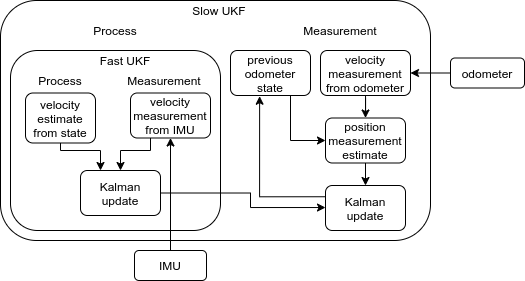
\includegraphics[width=0.9\textwidth]{figures/dukf.png}
    \caption{Double UKF data flow model}
    \label{fig:dukf}
\end{figure}

Every real world system deals with uncertainty in its processes and measurement data, which makes it difficult to accurately estimate a system's state, i.e. the important variables that describe a system in the world. Kalman filters solve the uncertainty problem with statistical probability representations of its state. Assuming that a state's uncertainty is approximately normally distributed, the essence of the state's expected values can be described by only keeping track of its mean and covariance. The Kalman filter updates the mean and covariance of the state over time using a dynamic Bayesian filter. Not only that, but if the process and measurement models are linear, the Kalman filter is the least squares approximator of the system, leading to optimal estimations of the state. 

In reality most systems are non-linear, and thus the standard Kalman filter has to be expanded to deal with process or measurement non-linearities. Two common approaches are model linearization, also known as the Extended Kalman filter (EKF), and the unscented transformation of specific state estimates, also known as the Unscented Kalman filter (UKF). This paper implements a UKF to solve sytem dynamics, as it is generally more accurate, but also because the UKF is well suited to the nature of the problem. The localization problem is framed in such a way to require two semi-independent filters, one fast and one slow. Yet the data should still be comparable between the models. By creating the sigma points in the slow filter and updating the systems belief based on those sigma points in the fast filter, the slow filter will have access to both the original data from the previous iteration and the update estimate from the fast filter. This simplifies the design process and enables the UKF to work correctly.

\textbf{UKF theory}

A UKF filters data by creating a set of sigma points from the state, which are processed to obtain an estimate of the current state of the system. This is statistically combined with an estimate from the measurement data to produce a new state estimate. The sigma points are used to reconstruct the distribution of the state after the non-linear transform, and thus each point is offset from the mean by a specific amount. The deviation, also known as weights $W$ are obtained by the Cholesky decomposition of the covariance $P$ with noise $Q$ of the state $x$. 

The Cholesky decomposition is effectively the square root of a matrix, and determines $L$, where $A=L^TL, L=\sqrt{A}$. Each position $(i,j)$ of $L$ can be calculated as

\begin{align}
    L_{ij} &= \left\{ \begin{array}{ll}
        \sqrt{A_{ij} - \sum_{k=0}^{j-1} L_{jk}^2} & \text{if } i = j \\
        \dfrac{1}{L_{jj}} \sqrt{A_{ij} - \sum_{k=0}^{j-1} L_{jk}^2} & \text{otherwise }
    \end{array}
    \right.
\end{align}

The set of sigma points $\{X_i\}$ are obtained as

\begin{align}
    W_i &= \text{columns}(\sqrt{2n \cdot (P_{k-1}+ Q}) & i &= 1...n \\
    W_{i+n} &= \text{columns}(-\sqrt{2n \cdot (P_{k-1}+ Q})  & i &= n+1...2n\\
    X_i &= \hat{x}_{k-1} + W_i & \text{i = $1$...$2n$}
\end{align}

where $n$ is the dimensionality of the state vector. The sigma are transformed through the non-linear process model $A(x, q)$ to obtain the processed points $\{Y_i\}$, as well as the measurement model $H(x, r)$, to obtain the measured points $\{Z_i\}$. The noise variables $q$ and $r$ are set to zero, as noise has already been added into the points as $Q$.

\begin{align}
    Y_i &= A(X_i, 0) \\
    Z_i &= H(X_i, 0) 
\end{align}

The mean and covariance of $\{Y_i\}$ and $\{Z_i\}$ are calculated as the weighted sum and correlation of the sets. The measurement noise $R$ is added to the measured covariance $P_{zz}$.

\begin{align}
    x_k^{-} &= \sum_{i=0}^{2n}W_i^{(m)} Y_i & z_k^{-} &= \sum_{i=0}^{2n}W_i^{(m)} Z_i \\
    P_k^{-} &= \sum_{i=0}^{2n}W_i^{(c)} \{Y_i - x_k^{-}\}\{Y_i - x_k^{-}\}^T & P_{zz,k} &= \sum_{i=0}^{2n}W_i^{(c)} \{Z_i - z_k^{-}\}\{Z_i - z_k^{-}\}^T \\
    & & P_{vv} &= P_{zz} + R
\end{align}

The Kalman gain $K_k$ represents the weighted degree of confidence the system has in the process and measurement models respectively, and is calculated with the cross-correlation of $\{Y_i\}$ and $\{Z_i\}$, $P_{xz}$, which aids in understanding how the process and measurement data influence each other.

\begin{align}
    P_{xz} &= \sum_{i=0}^{2n}W_i^{(c)} \{Y_i - x_k^{-}\}\{Z_i - z_k^{-}\}^T \\
    K_k &= P_{xz} P_{vv}^{-1}
\end{align}

Finally the mean and covariance of the system can be updated as the Kalman weighted sum of the process and measurement estimate.

\begin{align}
    x_k &= x_k^{-} + K_k (z - z_k^{-}) \\
    P_k &= P_k^{-} - K_k P_vv K_k^T
\end{align}

\textbf{Fast UKF Process model}

\textbf{Slow UKF Process Model}

\subsubsection{Mapping}
\label{sec:mapping}

Localization by itself does not present the robot with enough information to act intelligently. The robot should have an idea about how the environment looks and works, not necessarily in extreme detail, but at least clear enough so that the robot can plan paths to specific goals and prevent collisions with obstacles in the environment. The robot needs a map, either as a point-based representation of obstacles or as a planar grid map describing the occupancy of each position.

The latter representation is known as an occupancy grid map, a two dimensional grid of cells, where each cell has a value between 0 (free) and 1 (occupied). Even though the graph represents binary occupancy, i.e. it assumes that each cell is either completely free or completely occupied, a cell's value will typical be a decimal value between the two extremes. This is necessary to account for the uncertainties in the sensor readings perceiving the environment. Sonar range technology as employed in this project can be quite inaccurate and is prone to outlier vulnerabilities. By storing the probability that a cell is occupied rather than just a zero or one, the system is more flexible to deal with uncertainties by updating the map based on recurrent consensus of the occupancy of a cell over time. The probabilistic representation of the map is also desirable as it can be processed with Bayesian filtering. 

Mapping large areas can quickly become large, complex problems. Therefore, to simplify the problem, we assume three things about the nature of the world and the map. First, it is assumed that every cell is either completely occupied or completely free, which is known as the occupancy assumption. Secondly, it is assumed that the world is static, no dynamic object except for the robot traverses the state space, which is known as the static assumption. Thirdly it is assumed that each cell is independent of one another, which is known as the independence assumption. It is clear that these assumptions do not always hold, a person can easily walk through the mapped area and it is quite reasonable to believe that some cells are partially covered or that the presence of an obstacle in one cell affects the probability of an obstacle in the next one. Fortunately the inaccuracies introduced by these assumptions are usually negligible, while the incorporation of these assumptions into the model produces a vastly simplified problem to solve.

\textbf{Static Binary Bayes Filter}

Given sensor data $z_{1:t}=\{z_1,z_2,...,z_t\}$ and input controls $u_{1:t}=\{u_1,u_2,...,u_t\}$, the objective of the mapping algorithm is to calculate the most likely map $m*$, where $m*$ is the maximum likelihood estimate of map given the input data:

\begin{align}
    m* &= \text{argmax}_m p(m|z_{1:t}, x_{1:t})
\end{align}

using the independence assumption $p(m_j|m_i) = p(m_j)$ for cells $i$ and $j$ in the map, the problem reduces to a joint probability or product of the individual cells, which can be expressed using Bayes rule,

\begin{align}
    p(m|z_{1:t},x_{1:t}) &= \prod_i p(m_i|z_{1:t},x_{1:t}) \\
    p(m_i|z_{1:t},x_{1:t}) &= \dfrac{p(z_t|m_i,z_{1:t-1},x_{1:t}) p(m_i|z_{1:t-1},x_{1:t})}{p(z_t|z_{1:t-1},x_{1:t})}
    \label{eq:bayes_rule}
\end{align}

which describes the probability that a cell is occupied given sensor data proportional to the probability of the sensor data given that the cell is occupied. A useful property of Bayesian network is the Markov assumption, which states that the future state of the system is conditionally independent of past states, given the current state. Thus, equation \ref{eq:bayes_rule} can be simplified by removing all past sensor data, $z_{1:t-1}$, given current data $z_t$ and by disregarding future input controls, $x_t$, given the current map $m_i$.

\begin{align}
    p(m_i|z_{1:t},x_{1:t}) &= \dfrac{p(z_t|m_i,x_t) p(m_i|z_{1:t-1},x_{1:t-1 })}{p(z_t|z_{1:t-1},x_{1:t})}
\end{align}

Bayes rule can be applied once again to the first term in the numerator, and multiplied back into the equation
 
\begin{align}
    p(z_t|m_i,x_t) &= \dfrac{p(m_i|z_t,x_t)p(z_t|x_t)}{p(m_i|x_t)} \\
    p(m_i|z_{1:t},x_{1:t}) &= \dfrac{p(m_i|z_t,x_t)p(z_t|x_t) p(m_i|z_{1:t-1},x_{1:t-1 })}{p(m_i|x_t)p(z_t|z_{1:t-1},x_{1:t})}
\end{align}

A few terms in this equation are difficult to estimate, such as $p(z_t|x_t)$, which estimates the probability of a sensor given a position with no mapping information, and $p(m_i|x_t)$, which estimates the probability of a cell's occupancy given a position without sensor data. The second term can be simplified by assuming the map is independent of a robot's position in the absence of sensor data, $p(m_i|x_t) = p(m_i)$, which represents the prior probability that any cell in a map is occupied. This prior would be high in a thickly crowded environment and low in an area with large open spaces.

As the occupancy grid map represents binary data, i.e. each cell is either occupied or free, the Bayesian filter for the opposite event is valid, and thus the ratio of the two probabilities can be expressed and simplified as:

\begin{align}
    p(\neg m_i|z_{1:t},x_{1:t}) &= \dfrac{p(\neg m_i|z_t,x_t)p(z_t|x_t) p(\neg m_i|z_{1:t-1},x_{1:t-1 })}{p(\neg m_i)p(z_t|z_{1:t-1},x_{1:t})} \\
    \dfrac{p(m_i|z_{1:t},x_{1:t})}{p(\neg m_i|z_{1:t},x_{1:t})} &= \dfrac{\dfrac{p(m_i|z_t,x_t)p(z_t|x_t)     p(m_i|z_{1:t-1},x_{1:t-1 })}{p(m_i)p(z_t|z_{1:t-1},x_{1:t})}}{\dfrac{p(\neg m_i|z_t,x_t)p(z_t|x_t) p(\neg m_i|z_{1:t-1},x_{1:t-1 })}{p(\neg m_i)p(z_t|z_{1:t-1},x_{1:t})}} \\
    &= \dfrac{p(m_i|z_t,x_t) p(m_i|z_{1:t-1},x_{1:t-1})p(\neg m_i)}{p(\neg m_i|z_t,x_t) p(\neg m_i|z_{1:t-1},x_{1:t-1}p(m_i)}
\end{align}

The occupancy assumption simplifies $p(\neg m_i) = 1 - p(m_i)$ as

\begin{align}
    \dfrac{p(m_i|z_{1:t},x_{1:t})}{1 - p(m_i|z_{1:t},x_{1:t})} &= \dfrac{p(m_i|z_t,x_t)}{1 - p(m_i|z_t,x_t)} \dfrac{p(m_i|z_{1:t-1},x_{1:t-1})}{1 - p(m_i|z_{1:t-1},x_{1:t-1})} \dfrac{(1 - p(m_i)}{p(m_i)}
    \label{eq:map_ratio_bayes}
\end{align}

From Equation \ref{eq:map_ratio_bayes} it is evident that the system consists of three parts. The $p(m_i|z_t,x_t)$ term describes the influence of the current sensor observation $z_t$, the $p(m_i|z_{1:t-1},x_{1:t-1})$ term describes the influence of the estimate from the previous state of the cell, and the $p(m_i)$ term describes the influence of the a priori information of the map, independent of sensor measurements.
 
Equation \ref{eq:map_ratio_bayes} currently describes the odds ratio $Odds(x) = \dfrac{p(x)}{1 - p(x)}$ of the probability. Using simple algebra the probability $p(x)$ can be recovered.

\begin{align}
    Odds(x) &= \dfrac{p(x)}{1 - p(x)} \\
    p(x) &= Odds(x) - Odds(x) p(x) \\
    p(x)(1 + Odds(x)) &= Odds(x) \\
    p(x) &= \dfrac{Odds(x)}{1 + Odds(x)} = \dfrac{1}{1 + \dfrac{1}{Odds(x)}}
\end{align}

which finally leads to the equation for $p(m_i|z_{1:t},x_{1:t})$,

\begin{align}
    p(x) &= [1 + Odds(x)^{-1}]^{-1} \\
    p(m_i|z_{1:t},x_{1:t}) &= \left[1 + \dfrac{1 - p(m_i|z_t,x_t)}{p(m_i|z_t,x_t)} \dfrac{1 - p(m_i|z_{1:t-1})}{p(m_i|z_{1:t-1},x_{1:t-1}),x_{1:t-1})} \dfrac{p(m_i)}{(1 - p(m_i)}\right]^{-1}
\end{align}

\textbf{Log-Odds Notation}

However, applying the latter equation to every cell in a grid map can quickly become computationally expensive, and given that the mapping algorithm has to coexists with other algorithms on a resource constrained microcontroller, it is imperative to optimize the algorithm even further.

First, let us define the log-odds of the probability of $x$ and its inverse as

\begin{align}
    l(x) &= \log \dfrac{p(x)}{1 - p(x)} & p(x) &= 1 - \dfrac{1}{1 + e^{l(x)}}
\end{align}

representing the map in log-odds space reduces the mapping equation to

\begin{align}
    l(m_i|z_{1:t},x_{1:t}) &= l(m_i|z_t, x_t) + l(m_i|z_{1:t-1}, x_{1:t-1}) - l(m_i) \\
    l_{t,i} &= h(m_i, x_t, z_t) + l_{t-1,i} - l_0
    \label{eq:logodds_recur}
\end{align}

where $h(x)$ is the measurement model that relates a new measurement to a log-odds probability. Equation \ref{eq:logodds_recur} clearly shows the recursive nature of the algorithm, as each update step just involves an addition of the new sensor data probability and a subtraction of the prior probability. Updating a log-odds map is fast, efficient and even allows parallelism, as none of the map cells are dependent on one another.

\textbf{Measurement model}

The map algorithm only updates the cells that are currently in the field of view of the sonar sensors, which emits a sonar signal in the form characterized in Figure \ref{fig:sonar_grid}.

\begin{figure}[H]
    \centering
    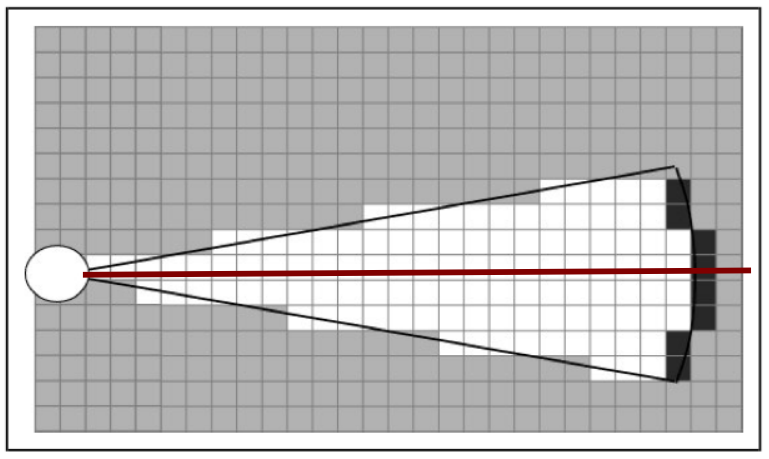
\includegraphics[width=0.7\textwidth]{figures/sonar_grid.png}
    \caption{Map grid cells in field of view of sonar sensor. Courtesy Burgard \cite{burgard_mr}.}
    \label{fig:sonar_grid}
\end{figure}

A few properties of the sensor is apparanet from Figure \ref{fig:sonar_grid}. Firstly, the sonar does not emit a directed beam in a specific direction, but has a deviation angle $\theta$ from which an emitted beam can be reflected back. Secondly, the sensor only detects the nearest object in its field of view (FOV), regardless of the view's width. This is can be shown by the arc of dark cells at the end of the beam, any of which can be the location of the real object. To deal with uncertainty in the measurement, a cell's modified probability depends on the cell's relative distance to the perceived obstacle and its deviation from the center of the sensor's orientation.

\begin{figure}
    \centering
    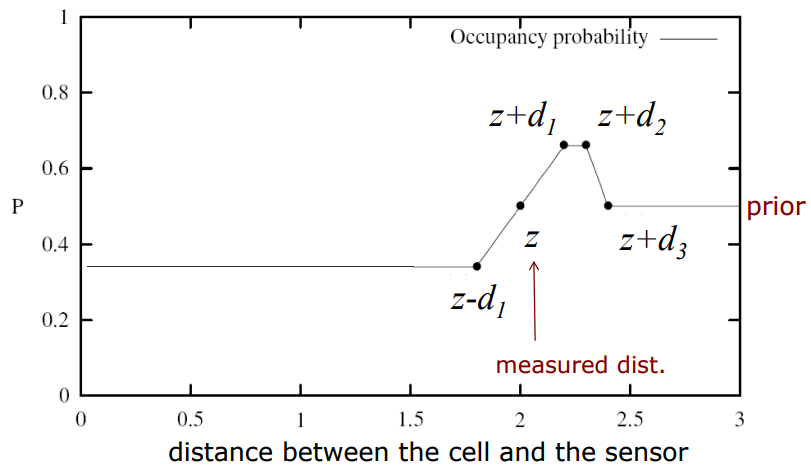
\includegraphics[width=0.8\textwidth]{figures/sonar_dist_p.png}
    \caption{Distance dependent probability update. Courtesy Burgard \cite{burgard_mr}.}
    \label{fig:sonar_dist_p}
\end{figure}

Figure \ref{fig:sonar_dist_p} describes the occupancy confidence of cells in the FOV, based on on where they are on the sensor distance line. The sensor confidence can be expressed in terms of constants $d_1, d_2, d_3$, which estimate the sensor noise and general thickness of obstacles. Cells that lay between $x_t$ and $z_t-d_1$ are perceived to be unoccupied, and will have a low probability, cells between $z_t-d_1$ and $z_t+d_1$ gradually increase in occupancy confidence as the measured distance approaches. Cells between $z_t+d_1$ and $z_t+d_2$ are regarded as obstructed, even with noise in the sensor it is reasonable to assume an obstruction $d_1$ further from the reading. Finally cells between $z_t+d_2$ and $z_t+d_3$ technically behind the sensed obstacle and thus no information about their occupancy is available. The same is true for cells beyond $z+d_3$. This can be evaluated in a piecewise function as

\begin{align}
    d &= \sqrt{(m_{i,x} - x_{t,x})^2 + (m_{i,y} - x_{t,y})^2} \\
    p(m_i) &= \left\{ \begin{array}{ll}
        p_{LOW} & d \leq z_t + d_1 \\
        p_{LOW} + \dfrac{p_{HIGH} - p_{LOW}}{2d_1} (d - z_t - d_1) & z_t-d_1 < d \leq z_t+d_1  \\
        p_{HIGH} & z_t+d_1 < d \leq z_t+d_2 \\
        p_{HIGH} - \dfrac{p_{HIGH} - p_0}{d_3 - d_2} (d - z_t+d_3) & z_t+d_2 < d \leq z_t+d_3 \\
        p_0 & d > z_t + d_3
    \end{array}
    \right.
\end{align}

\begin{figure}
    \centering
    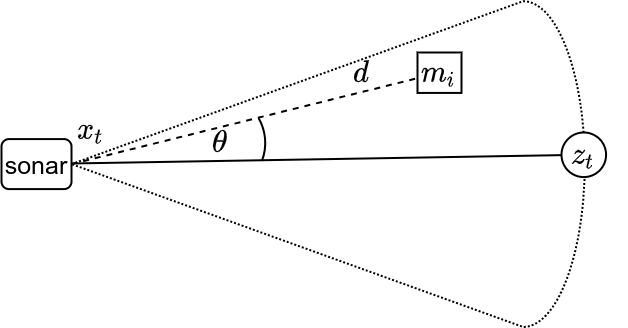
\includegraphics[width=0.7\textwidth]{figures/sonar_angle_p.png}
    \caption{Angle dependent probability update. Courtesy Burgard \cite{burgard_mr}.}
    \label{fig:sonar_angle_p}
\end{figure}

Figure \ref{fig:sonar_angle_p} shows a cell that is deviated from the center of the sonar's FOV by $\theta$. Assuming that sensor readings at a deviated angle will be less accurate and more prone to errors, it is wise to multiply the proposed confidence with a Gaussian distributed weight around the deviation $\theta$. The probability density function $f(x)$ of a normally distributed set equates to

\begin{align}
    f(x) &= \dfrac{1}{\sigma\sqrt{2\pi}} e^{-\dfrac{(x - \mu)^2}{2\sigma^2}}
\end{align}

with standard deviation $\sigma$ and mean $\mu = 0$, which can be used to calculate the Gaussian weight $s_\theta$ as

\begin{align}
    s_\theta &= \left\{ \begin{array}{ll}
        \dfrac{1}{\sigma\sqrt{2\pi}} e^{-\dfrac{\theta^2}{2\sigma^2}} & \theta \leq 0 \\
        \dfrac{1}{\sigma\sqrt{2\pi}} e^{-\dfrac{(1 - \theta)^2}{2\sigma^2}} & \theta > 0
    \end{array}
    \right.
\end{align}

Finally the measurement model can be expressed as

\begin{align}
    h(m_i, x_t, z_t) &= \log \dfrac{s_\theta p(m_i)}{1 - s_\theta p(m_i)}
\end{align}

Modern approaches tend to integrate the localization and mapping problems in one of several SLAM algorithms. This approach was not pursued intentionally as those algorithms require a lot of computational power and quite accurate distance readings. The proposed system has neither, working with a low-end microcontroller and low quality sonar sensors, but rather maps the world with known poses, thus it assumes localization is fairly accurate. The focus now shifts from a highly complex simultaneous optimization problem to ensuring accurate positioning, which is done through the incorporation of three different sensors in a sophisticated UKF for precise state estimation.

\subsubsection{Control}
\label{sec:control}

The passive aspects of the system have been dealt with, and the robot can effectively estimate its position and perceive the environment, but so far it is unable to plan paths nor act on those plans. In this section we assume a path has already been determined, and investigate the methods the robot employs to reach this goal accurately and timely.

The simplest control model aims to reach a desired state $x'$ from its current state $x$ by sending a set of controls $u$ to its actuators, producing state $y$. This model does not incorporate any perceptual information about the environment and is an open loop controller. This model is vastly insufficient for any system operating in the real world, as it does not account for noise, faulty actuators or dynamic unexpected events. A better model also incorporates sensor data to update the estimate of its state in what is known as a closed loop feedback controller.

\begin{figure}[H]
    \centering
    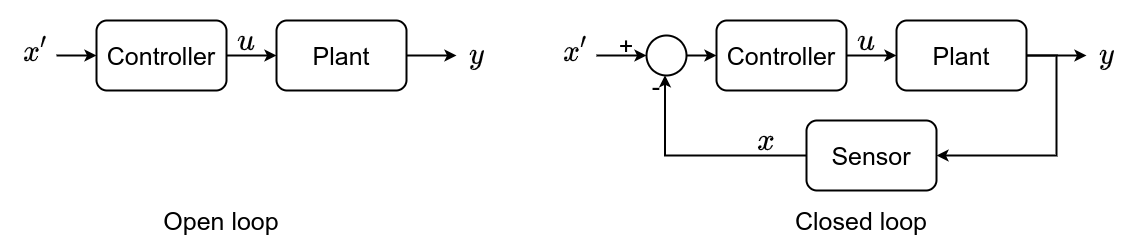
\includegraphics[width=\textwidth]{figures/open_loop.png}
    \caption{Open loop vs. closed loop controller}
    \label{fig:open_loop}
\end{figure}

A closed loop controller continually uses sensor data to update the error, $e$, between the desired and current states. The data flow model for a closed loop controller is given in Figure \ref{fig:closed_loop}, showing the interaction between the desired state $x_t'$, the current state $x_t$, the measured state $z_t$ and the input controls $u_t$. Process nosie $\epsilon_t$ and measurement noise $\delta_t$ also affect the system. The controller's objective is to relate the error between the desired and current state to the required input controls that will eventually result in the robot reaching the goal.

\begin{figure}[H]
    \centering
    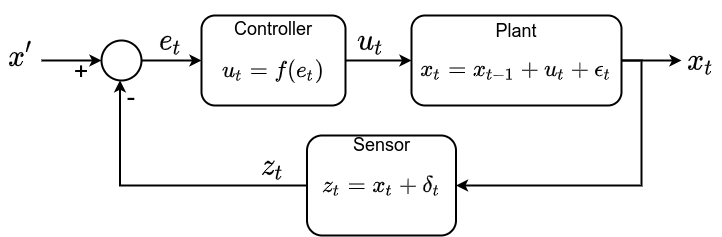
\includegraphics[width=0.8\textwidth]{figures/closed_loop.png}
    \caption{Closed loop controller data flow model}
    \label{fig:closed_loop}
\end{figure}

\textbf{PID controller theory}

Let us first examine a generic feedback controller with the above-mentioned parameters. The simplest controller would set the input proportional to the error,

\begin{align}
    u_t &= K_p (x' - x_t) \\
    &= K_p e_t, K_p < 1
    \label{eq:p-control}
\end{align}

where $K_p$ is the proportionality constant. Limiting $K_p$ to be less than one ensures that the system produces an input smaller than its perceived error, leading to a stable system response. On the other hand, if $K_p > 1$ the system would produce input larger than the error, which can lead to positive feedback and instability. 

The controller in Equation \ref{eq:p-control} works theoretically, but three physical phenomenon can degrade the quality of the system response. Firstly, the system is susceptible to noise, both in the actuators and in the sensors, which can lead to oscillations around the desired goal state, second a delay between the system's response and its perception of the reponse can lead to overcompensation for an action that has already been adjusted for, but due to inertia or sensor characteristics the effect is not seen yet. Thirdly, in the case where the system controls for the rate of change of a particular variable, such as the velocity of the robot's position, just reaching the desired position is not sufficient, as the system's velocity will cause it to overshoot. Rather the system should act in a manner to compensate for both its state and the rate of change of the state, to reach the goal state and remain there.

Noise and delay can be reduced by setting a lower value of $K_p$, but it can lead to a slower convergence rate. This is effectively a trade-off between fast convergence and low steady-state error, depending on the design requirements. In the latter case the system can be modelled more accurately according to Equation \ref{eq:pd-model}, accounting for both its state and its rate of change or derivative. This will ensure that the input is not only dependent on the magnitude of the error, but also the rate at which we are reducing the error, to ensure low oscillatory behaviour in the vicinity of the goal. As a bonus, the introduction of a derivative term facilitates the use of a larger stable proportional constant, leading to faster convergence.

\begin{align}
    x_t &= x_{t-1} + \Dot{x}\Delta t
    \label{eq:pd-model} \\
    u_t &= K_p (x' - x_t) + K_d (\Dot{x}' - \Dot{x}_t) \\
    u_t &= K_p e_t + K_d \dfrac{de_t}{dt}
\end{align}

A final modification can be made to the controller by considering the problem of steady state errors. These are small errors in the state when in the vicinity of the goal that accumulate over time to take the system off course. This is, for example, applicable if the desired state is a certain velocity to reach a faraway target, but due to a small deviation the target is not reached. Steady state errors are usually small enough that the proportional controller do not correct for them, or at least cannot do so effectively, as it is designed to deal with large inaccuracies. The solution is to correct for the integral of the error over time as part of the controller.

\begin{align}
    u_t &= K_p (x' - x_t) + K_d (\Dot{x}' - \Dot{x}_t) + K_i \int_0^t (x' - x_t) dt \\
    u_t &= K_p e_t + K_d \dfrac{de_t}{dt} + K_i \int_t e_t dt
\end{align}

The introduction of the integral term does however put the system in danger of the error build up, also known as the wind-up effect. If the robot does not act in the way it ought to, according to its model, which can happen if it is for example stuck in a hole. The integral error will continue to increase dramatically and completely disrupt the system once the robot comes out of the hole. The solution is to only integrate the error over fixed periods of time instead of over all possible time, which will at least contain the integral error to an upper manageable limit.

\textbf{Motor control}

With the theoretical foundation laid, we can proceed to the mathematical models of the motor and position controllers. The motor controller restricts its operation to the performance and expectation of the motors, and aims to reduce the error between the real and desired translational and rotational velocities $(v,\omega)$. This controller not only assumes that the desired position is known, but also that the position controller, described below, established the required velocities $(v,\omega)$ to reach the goal. The motivation for the separation of the two systems is that it produces a two modular, independent software components that can function semi-independent of one another, which eases development, debugging and maintenance. For the motor controller this allows a simplistic and focused model, and for the position controller this abstracts away the physical implementation of the velocities, once again simplifying and focusing its model.

The motor controller has state $\mathbf{x} = \{v, \omega\}$, where $v$ describes the forward velocity and $\omega$ the angular velocity of the robot. The desired state is of the same form $\mathbf{x}' = \{v', \omega'\}$. The input controls are the duty cycles that drive the PWM of the left and right motors, $\mathbf{u} = \{u_l, u_r\}$, and must have a value between -1 and 1. The sensors are the light-based odometers attached to the shafts of each wheel, which record the amount of holes $n$ in a wheel encoder that passes by in a specific time frame $\Delta t$. This is easily converted angular velocity of the wheel, $\omega_i$, and forward velocity, $v_i$, as

\begin{align}
    d_i &= r\omega_i = \dfrac{2 \pi r n}{N \Delta t} \\
\end{align}

with $N$ the total amount of holes in the encoder and $r$ the radius of the wheels. The error forward and angular velocity is calculated as $\mathbf{e}=\{e_v, e_\omega\}$, using the chassis length $l$. The motor controller implements a simple proportional controller in as Equation \ref{eq:p-control-motor}.

\begin{align}
	e_v &= v' - \dfrac{v_r + v_l}{2} & e_\omega &= \omega' - \dfrac{v_r - v_l}{l} \\
    \begin{bmatrix} u_r \\ u_l \end{bmatrix} &= K_p \begin{bmatrix}
        1 & K_\omega \\
        1 & -K_\omega
    \end{bmatrix} \begin{bmatrix}
        e_v \\ e_\omega
    \end{bmatrix}
    \label{eq:p-control-motor}
\end{align}

In essence the controller uses the translational velocity to set a velocity bar for both wheels, which is offset one way or another depending on the direction and magnitude of the desired angular velocity.

\textbf{Position control}

The position controller aims to move the robot from its current position to its desired position by dynamically updating the required translational and angular velocities needed to get there with a PID-controller. The controller has state $\mathbf{x} = \{x, y, \theta\}$, describing the current position and orientation of the robot in 2D state space, as well as desired state $\mathbf{x}'=\{x', y'\}$ as the goal and $\mathbf{u} = \{v, \omega\}$ as the input controls to the motor controller.

The first step is to obtain the distance and angular offset error between the current and desired state, which effectively converts the error to polar form.

\begin{align}
    e_t &= f(\mathbf{x}' - \mathbf{x}) \\
    \begin{bmatrix} e_r \\ e_\theta \end{bmatrix} &= \begin{bmatrix}
        \sqrt{(x' - x)^2 + (y' - y)^2} \\
        \text{atan2}(y' - y, x' - x) - \theta
    \end{bmatrix}
\end{align}

the C function \texttt{atan2()} is used as it respect the sign of the angle. Using the previous error states $e_{1:t-1}$, the integral and derivative terms can be calculated as

\begin{align}
    \int_0^t e_t d_t &= \sum_{i=0}^t e_i \Delta t = \sum_{i=0}^{t-1} e_i \Delta t + e_t \Delta t \\
    \dfrac{de_t}{dt} &= \dfrac{e_t - e_{t-1}}{\Delta t}
\end{align}

where the $\sum_{i=0}^{t-1} e_i \Delta t$ is the sum of all previous errors up to $e_{t-1}$ and is updated recursively. Finally the PID-controller can be implemented as

\begin{align}
    u_t &= K_p e_t + K_i \int_0^t e_t dt + K_d \dfrac{de_t}{dt} \\
    \begin{bmatrix} u_v \\ u_\omega \end{bmatrix} &= 
    \begin{bmatrix} K_{p,r} \\ K_{p,\theta} \end{bmatrix}
    \begin{bmatrix} e_{t,r} \\ e_{t,\theta} \end{bmatrix} +
    \begin{bmatrix} K_{i,r} \\ K_{i,\theta} \end{bmatrix}
    \begin{bmatrix} \int_0^t e_{t,r} dt \\ \int_0^t e_{t,\theta} dt \end{bmatrix} +
    \begin{bmatrix} K_{d,r} \\ K_{d,\theta} \end{bmatrix}
    \begin{bmatrix} \Dots{e}_{t,r} \\ \Dots{e_{t,\theta}} \end{bmatrix} 
\end{align}

\subsubsection{Path planning}
\label{sec:path-plan}

\subsubsection{Navigation}
\label{sec:navigation}

\subsection{Simulations}
\label{sec:sim}

\subsection{Hardware Design and Implementation}

\subsubsection{Sensors}
\label{sec:sensors}

The autonomous vacuum cleaner has to interact with the environment in an intelligent manner, having knowledge of the landscape as well as its own observed actions. Thus, choosing the sensor components that will give real-time measurement input to the system is an integral first step in the journey towards robotic perception. The required input data aims to update the robot's perception of reality primarily in two ways: input that tells the robot about the environment, and input that observes the robot's actions. \\

The sensor input that describes the environment has to quantify the landscape by measuring the distance to obstacles in the horizontal plane close to the floor. Ideally the robot should be able to get a sense of the position of a measured obstacle relative to itself, thus both the distance to and the approximate direction of the obstacle is required. The potential sensor candidates include Lidar sensors, cameras, ultrasonic sensors and infrared scanners. \\

After thorough research and requirements evaluation it became clear that HC-SR04 ultrasonic sensors are the most suitable candidate for the system. An ultrasonic sensor is a distance sensing device that contains a transmitter and a receiver used to emit and receive an ultrasonic pulse respectively. Transmission of a 40kHz signal pattern starts while an echo pin is simultaneously pulled high until the transmitted pulse is reflected back into the receiver module. Measuring the length of the travelling pulse, while assuming that the speed of sound is known and approximately constant, the distance to the nearest obstacle in the direction of the sensor can easily be determined. The sensor does however have a $30^\circ$ total angular range or field of view within which the closest object will be detected. This leads to uncertainty in the exact location of the obstacle, as any position in a arc around the sensor's view could produce a reading at the specific distance. Despite this challenge, which will be addressed later on, the ultrasonic sensor is still the best sensor for the job due to the little post-processing required to interpret its measurement data, its large measurement range (2cm - 4m), its ability to operate in low lighting conditions and its relatively low power consumption, which is important for a system that runs on batteries. \\

\begin{figure}[H]
    \centering
    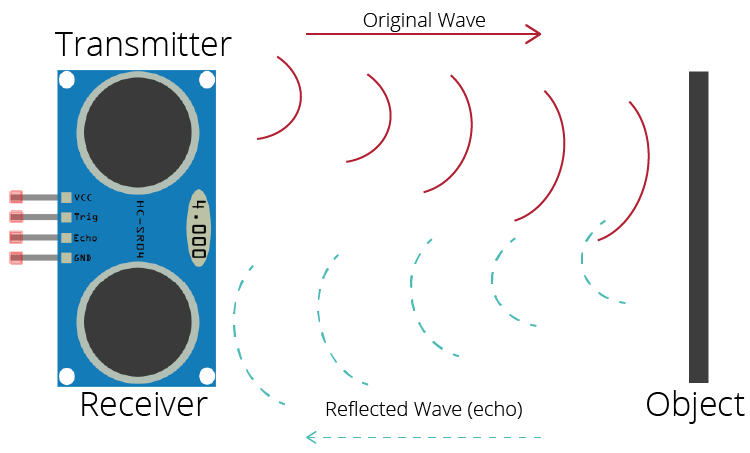
\includegraphics[width=0.5\textwidth]{figures/hcsr04_waves.png}
    \caption{HC-SR04 ultrasonic wave operation}
    \label{fig:hcsr04_waves}
\end{figure}

The system implements three HC-SR04 sensors in a semi-circle around the front of the robot, placed at such an angle that the three sensors collectively scan a $120^\circ$ field of view directly ahead of the robot, with each sensor placed offset by $40^\circ$ relative to one another. The $10^\circ$ blind spot produced by this design is small enough that it is highly unlikely that an obstruction can hide in there, without showing up in measurement readings on either side of the gap, especially across different samples taken at different locations. \\

A glaring limitation prohibits the use of higher resolution sensor components, such as cameras or lidar, which is the amount of processing power and more importantly, memory, required to effectively analyse incoming data. Computer vision algorithms are bulky and expensive, requiring tens of thousands of matrix operations and several levels of filtering, processing and AI-based sorting to work. These approaches are unfeasible for the simple, low-cost solution that this project aims to implement. Memory is a particularly constrained resource in an embedded system, with every single byte of stored space important. An array of photos in different processing stages taking up a few megabytes of storages is simply not an option. \\

The second set of sensors address the potential non-determinism in the robot's expected actions. The robot navigates the world by setting the duty cycle of the motors turning the wheels. This action is quite simple, but prone to process noise. For example, if both motors receive the same PWM duty cycle, the expected outcome is forward propagation in a straight line, but due to differences in friction, magnetic field strength and physical construction, one of the motors inevitable turns a little bit faster than the other one, which slowly takes the robot off course until it finds itself in a completely different location and orientation than its internal map of the world expects it to be. \\

The solution to actuator uncertainty involves an observation feedback loop coupled with a PI-controller, which will be explored in another section. The observation feedback loop observes properties of the robot that directly or indirectly provides information about the state of the device. These measurements are fused with the robots own estimation of its state to produce an updated state. Five sensor components are chosen for this task, a gyroscope, accelerometer and magnetometer combined in a 9-DOF IMU, as well as two odometers placed on the left and right wheels of the robot. Together these sensors can measure angular rate, velocity, acceleration and magnetic induction in three dimensions, potentially providing more than enough information to correct the robot's estimate of its state. \\

As the robot only operates on a 2D plane, assuming that the robot will never fall of a cliff (not that accurate positioning will be of much use in that case in anyway), we can neglect measurement data in certain dimensions, such as the roll and pitch of the gyroscope and the gravitational tug in the vertical direction from the accelerometer. This simplifies the sensor fusion algorithms as we focus on the sensor data that have a real impact on the positioning of the robot. \\

In summary, the gyroscope, accelerometer and magnetometer of the MPU9250 IMU sensor works in conjunction with two light emitting odometers attached to the wheels to accurate estimate the position of the robot in its internal map of the world. Unfortunately the accelerometer has to be placed on an exactly level plane to prohibit gravity from affecting the readings on the horizontal plane. The gyroscope is also infamous for large amounts of bias and bias instability, leading to wildly inaccurate readings. To overcome both of these problems, the robot stays in an initialization state for three seconds upon startup, during which at least 30 IMU sensor measurement are taken. As the robot is assumed to be stationary, any deviation from the expected values can be interpreted as bias. The average of the measured bias is subsequently subtracted from every measurement taken during navigation. This relaxes the requirement for a flat accelerometer and accurate gyroscope, and experimental results prove that this simple bias removal technic vastly improves the accuracy of the measurement model state estmation.

\subsubsection{Veroboard}
\label{sec:veroboard}

The veroboard design initially started out as a desperate attempt to build a working prototype after several iterations of PCB boards failed to work. As veroboards are a lot easier to change, redo and improve, a design choice was taken to stick to veroboard prototyping. The veroboard is home to a small ecosystem of components, each playing their part in making the system work as a whole. \\

The most important component on the board is the PIC32MX270F256-B microcontroller from Microchip, boasting a 40 MHz clock, 256kB of flash memory and 64kB of SRAM, as well as the MIPS32 RISC architecture. The chip has 28 pins, of which 17 can be used as general purpose input/output (GPIO) pins. With 14 peripheral devices, some requiring more than one pin, it seemed impossible to reconcile the large peripheral need with the low pin count. Fortunately, through a mixture of iteration, optimization and careful design, creative methods were developed to squeeze as much functionality out of the pins as possible. \\

For example, originally the three ultrasonic distance sensors each had to be triggered by a separate trigger pin to start a distance reading, while the measurement occured on another separate echo pin. Thus 6 out of 28 pins were wasted on one aspect of the peripheral components. Then it was discovered that the same echo pin can be reused if the correct assortment of diodes and resistors are used to pull the line low between readings and to eliminate power loss on the shared bus. So now we are down to three trigger pins and one echo pin. Triggering all three pins at once will result in potential crosstalk between the sensors and should be avoided. Finally it was found that triggering a pin and listening to an echo has the same characteristic pulse on a line, thus if the echo pin of sensor 1 is connected to the trigger pin of sensor 2, a completed measurement on sensor 1 will automatically start transmission on sensor 2. This was the final breakthrough that allowed the system to dedicate only 2 pins to all three ultrasonic sensors, while simplifying the code necessary to operate these components. \\

Another example is the sharing of the I$^2$C bus. The IMU, magnetometer and OLED display screen communicate via I$^2$C. Thus by connecting the three components to the same two wires can be used for SDA and SCL, using I$^2$C addressing to announce the recipient of a message. Lastly, further optimization took place by only dedicating one pin, TX to the UART, as it is assumed that the robot will not receive any data but will only be used to display information. \\

\subsubsection{Robot body}
\label{sec:robot} 

\subsubsection{Power management}
\label{sec:power}

Part of the design requirements of the robot describes the need to autonomously manage the robot's power consumption, whereby it returns back to the docking station (or starting location) once it detects low battery capacity. The robot can detect remaining capacity by measuring the voltage over the batteries. A single 18650 battery is fully charged at 4.2V, nominal at 3.7V and flat at 3.2V. The system has three 18650 batteries in series, thus it will be fully charged at 12.6V and dead at 9.6V. We would ideally want to halt operation and return back to the charger if the battery falls below 25\%, i.e. measured voltage is $<$ 10.2V. Of course, measuring voltages around 12V will completely fry a 3.3V chip, whereas simply lowering the voltage in a voltage divider will cause the applicable voltage range to be very small (2.5V - 3.3V). \\

Instead, the nature of electricity flow in the robot is used. The L298N H-bridge draws power from the batteries at their current varying voltage, but always outputs 5V to the veroboard circuit. By taking the scaled voltage difference between battery voltage and the 5V from the H-bridge in a differential amplifier, the complete range of the battery can be estimated more accurately.

\subsubsection{Vacuum pump}
\label{sec:vacuum}

\subsection{Software Design and Implementation}

\subsubsection{Peripheral drivers}
\label{sec:periph}

\subsubsection{Positioning and Sensor Fusion}
\label{sec:position}

\subsubsection{Mapping}
\label{sec:mapping}

\subsubsection{Motor Control}
\label{sec:control}

\subsubsection{Navigation}
\label{sec:navigation}



\subsubsection{Cleaning integration}
\label{sec:cleaning}

\subsection{Visual and statistical analysis}
\label{sec:stats}

\newpage

%% End of File.

%%
%%  Department of Electrical, Electronic and Computer Engineering.
%%  EPR400/2 Final Report - Section 3.
%%  Copyright (C) 2011-2021 University of Pretoria.
%%

\section{Design and implementation}

\subsection{Design summary}

This section summarises the project design tasks and how they were implemented (see table \ref{tab:design_sum}).

\begin{longtable}[H]{|p{0.28\textwidth}|p{0.4\textwidth}|p{0.28\textwidth}|} \hline
    \textbf{Deliverable or task} & \textbf{Implementation} & \textbf{Completion of deliverable or task, and section in the report} \\ \hline
    Determine sensor input requirements & 
    It was determined that the system needs 3 ultrasonic sensors to perceive distance, 2 infrared sensors to detect fall hazards, and a 9-DOF IMU and 2 light odometers to calculate the vehicle's position &
    Completed. Section \ref{sec:sensors} \\ \hline
    Design the hardware layout on the robot's motherboard &
    The original PCB design was replaced with a veroboard, which was iteratively optimized through first principles to design and build a small and efficient board & 
    Completed. Section \ref{sec:veroboard} \\ \hline
    Design and construct robot body &
    The robot chassis, motors, wheels, vacuum pump, board and sensors were integrated together in a small autonomous vehicle. & 
    Completed. Section \ref{sec:robot} \\ \hline
    Design and construct vacuum pump &
    The vacuum pump itself is an off-the-shelf hand vacuum, but the integration with the system, including current limiting breakout circuit was designed to control its operation during cleaning. &
    Completed. Section \ref{sec:vacuum}. \\ \hline
    Initialize and test peripherals &
    Peripheral drivers were developed from first principles for the PIC32 microcontroller, for the most efficient implementation and lowest possible latency. &
    Completed. Section \ref{sec:periph} \\ \hline
    Design and implement positioning algorithm &
    A positioning algorithm was implemented from first principles using complementary sensor fusion to position the robot on an internal 2D cartesian map. &
    Completed. Section \ref{sec:position} \\ \hline
    Design and implement navigation algorithm &
    A navigation algorithm was implemented from first principles using ultrasonic proximity detection to reach specific goals and avoid obstacles, as well as control movement intelligently. &
    Completed. Section \ref{sec:navigation} \\ \hline
    Design and implement mapping algorithm &
    A mapping algorithm was implemented from first principles to store visited and obstacle information from the environment to plan routes more effectively. &
    Completed. Section \ref{sec:mapping} \\ \hline
    Implement fall-protection algorithm &
    A simple maneuver to avoid large was developed with mixed success and will not be demoed extensively for the vehicle's safety. &
    Incomplete. \\ \hline
    Implement dirt-detection algorithm &
    The proposed dirt detection solution would have been too complex to incorporate into the system design, without adding any real value, and thus a design choice was taken to not implement this aspect of the system. &
    Incomplete. \\ \hline
    Implement autonomous power management algorithm & 
    An power management algorithm was implemented so that the robot returns to its starting position once it detects low power, but the docking station and mechanics of docking precisely was not implemented. &
    Incomplete. \\ \hline
    Integrate in floor-cleaning system &
    The integration of the positioning, navigation and mapping algorithms cleans a given floor area. &
    Completed. Section \ref{sec:cleaning} \\ \hline
    Test and verify results &
    A range of simulations and experiments were carried out to verify that the robot fulfills the specified requirements, including Python simulations, visual inspection and offline statistical analysis of positioning and navigation data. &
    Completed. Sections \ref{sec:sim} \& \ref{sec:stats} \\ \hline
    \caption{Design summary}
    \label{tab:design_sum}
\end{longtable}

\subsection{Theoretical background}
\label{sec:theory}

The mathematical structure of the robot's intelligent interaction with the environment can be divided into 5 subsystems: localization, mapping, control, path planning and navigation, working together to sense and perceive the environment, plan a goal and act to attain the goal.

\subsubsection{Localization}
\label{sec:localize}

\textbf{Filter motivation}

It is important for the robot to localize itself accurately in its internal representation of the world, as the success of the mapping and collision-free navigation depends on this. Localization is performing through the non-linear sensor fusion of the IMU's measured acceleration and gravity, as well as the measured wheel velocity from the odometers. A design choice was taken not to implement a SLAM algorithm, as multiple localize-only sensors are available to correct for noise and drift, and the sensors used for mapping, the sonar sensors, are quite inaccurate and do not produce a high quality map of the environment, which would make it difficult to use the mapping data successfully in localization. 

Instead a double Unscented Kalman Filter (UKF) is implemented complementing the nature of the sensors and their operation. The IMU can provide a quick succession of angular rate and acceleration values, and due to the transient nature of acceleration, these readings are also most accurate if obtained as continuously as possible. On the other the odometer needs time to measure the rotation of trotation of the wheel, and preemptively extrapolating the wheel spin leads to inaccuracies. 

Combining the strenghts and understanding the shortfalls of the two sensors, we propose a double UKF localization solution. The first filter, known as the "fast" filter, operates at 40 Hz, with its velocity estimate as the process model and incoming IMU data as the measurement model. The second "slow" filter operates at 4 Hz, using the last fast filter estimate as the process model and the incoming odometer readings as the slow filter. The double UKF data flow model is shown in Figure \ref{fig:dukf}.

\begin{figure}
    \centering
    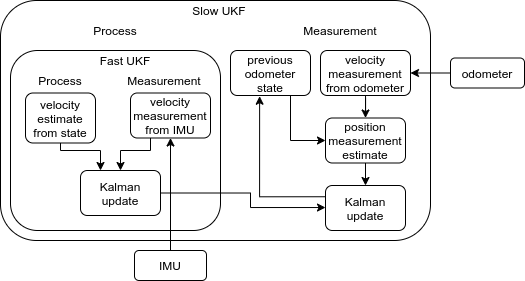
\includegraphics[width=0.9\textwidth]{figures/dukf.png}
    \caption{Double UKF data flow model}
    \label{fig:dukf}
\end{figure}

Every real world system deals with uncertainty in its processes and measurement data, which makes it difficult to accurately estimate a system's state, i.e. the important variables that describe a system in the world. Kalman filters solve the uncertainty problem with statistical probability representations of its state. Assuming that a state's uncertainty is approximately normally distributed, the essence of the state's expected values can be described by only keeping track of its mean and covariance. The Kalman filter updates the mean and covariance of the state over time using a dynamic Bayesian filter. Not only that, but if the process and measurement models are linear, the Kalman filter is the least squares approximator of the system, leading to optimal estimations of the state. 

In reality most systems are non-linear, and thus the standard Kalman filter has to be expanded to deal with process or measurement non-linearities. Two common approaches are model linearization, also known as the Extended Kalman filter (EKF), and the unscented transformation of specific state estimates, also known as the Unscented Kalman filter (UKF). This paper implements a UKF to solve sytem dynamics, as it is generally more accurate, but also because the UKF is well suited to the nature of the problem. The localization problem is framed in such a way to require two semi-independent filters, one fast and one slow. Yet the data should still be comparable between the models. By creating the sigma points in the slow filter and updating the systems belief based on those sigma points in the fast filter, the slow filter will have access to both the original data from the previous iteration and the update estimate from the fast filter. This simplifies the design process and enables the UKF to work correctly.

\textbf{UKF theory}

A UKF filters data by creating a set of sigma points from the state, which are processed to obtain an estimate of the current state of the system. This is statistically combined with an estimate from the measurement data to produce a new state estimate. The sigma points are used to reconstruct the distribution of the state after the non-linear transform, and thus each point is offset from the mean by a specific amount. The deviation, also known as weights $W$ are obtained by the Cholesky decomposition of the covariance $P$ with noise $Q$ of the state $x$. 

The Cholesky decomposition is effectively the square root of a matrix, and determines $L$, where $A=L^TL, L=\sqrt{A}$. Each position $(i,j)$ of $L$ can be calculated as

\begin{align}
    L_{ij} &= \left\{ \begin{array}{ll}
        \sqrt{A_{ij} - \sum_{k=0}^{j-1} L_{jk}^2} & \text{if } i = j \\
        \dfrac{1}{L_{jj}} \sqrt{A_{ij} - \sum_{k=0}^{j-1} L_{jk}^2} & \text{otherwise }
    \end{array}
    \right.
\end{align}

The set of sigma points $\{X_i\}$ are obtained as

\begin{align}
    W_i &= \text{columns}(\sqrt{2n \cdot (P_{k-1}+ Q}) & i &= 1...n \\
    W_{i+n} &= \text{columns}(-\sqrt{2n \cdot (P_{k-1}+ Q})  & i &= n+1...2n\\
    X_i &= \hat{x}_{k-1} + W_i & \text{i = $1$...$2n$}
\end{align}

where $n$ is the dimensionality of the state vector. The sigma are transformed through the non-linear process model $A(x, q)$ to obtain the processed points $\{Y_i\}$, as well as the measurement model $H(x, r)$, to obtain the measured points $\{Z_i\}$. The noise variables $q$ and $r$ are set to zero, as noise has already been added into the points as $Q$.

\begin{align}
    Y_i &= A(X_i, 0) \\
    Z_i &= H(X_i, 0) 
\end{align}

The mean and covariance of $\{Y_i\}$ and $\{Z_i\}$ are calculated as the weighted sum and correlation of the sets. The measurement noise $R$ is added to the measured covariance $P_{zz}$.

\begin{align}
    x_k^{-} &= \sum_{i=0}^{2n}W_i^{(m)} Y_i & z_k^{-} &= \sum_{i=0}^{2n}W_i^{(m)} Z_i \\
    P_k^{-} &= \sum_{i=0}^{2n}W_i^{(c)} \{Y_i - x_k^{-}\}\{Y_i - x_k^{-}\}^T & P_{zz,k} &= \sum_{i=0}^{2n}W_i^{(c)} \{Z_i - z_k^{-}\}\{Z_i - z_k^{-}\}^T \\
    & & P_{vv} &= P_{zz} + R
\end{align}

The Kalman gain $K_k$ represents the weighted degree of confidence the system has in the process and measurement models respectively, and is calculated with the cross-correlation of $\{Y_i\}$ and $\{Z_i\}$, $P_{xz}$, which aids in understanding how the process and measurement data influence each other.

\begin{align}
    P_{xz} &= \sum_{i=0}^{2n}W_i^{(c)} \{Y_i - x_k^{-}\}\{Z_i - z_k^{-}\}^T \\
    K_k &= P_{xz} P_{vv}^{-1}
\end{align}

Finally the mean and covariance of the system can be updated as the Kalman weighted sum of the process and measurement estimate.

\begin{align}
    x_k &= x_k^{-} + K_k (z - z_k^{-}) \\
    P_k &= P_k^{-} - K_k P_vv K_k^T
\end{align}

\textbf{Fast UKF Process model}

\textbf{Slow UKF Process Model}

\subsubsection{Mapping}
\label{sec:mapping}

Localization by itself does not present the robot with enough information to act intelligently. The robot should have an idea about how the environment looks and works, not necessarily in extreme detail, but at least clear enough so that the robot can plan paths to specific goals and prevent collisions with obstacles in the environment. The robot needs a map, either as a point-based representation of obstacles or as a planar grid map describing the occupancy of each position.

The latter representation is known as an occupancy grid map, a two dimensional grid of cells, where each cell has a value between 0 (free) and 1 (occupied). Even though the graph represents binary occupancy, i.e. it assumes that each cell is either completely free or completely occupied, a cell's value will typical be a decimal value between the two extremes. This is necessary to account for the uncertainties in the sensor readings perceiving the environment. Sonar range technology as employed in this project can be quite inaccurate and is prone to outlier vulnerabilities. By storing the probability that a cell is occupied rather than just a zero or one, the system is more flexible to deal with uncertainties by updating the map based on recurrent consensus of the occupancy of a cell over time. The probabilistic representation of the map is also desirable as it can be processed with Bayesian filtering. 

Mapping large areas can quickly become large, complex problems. Therefore, to simplify the problem, we assume three things about the nature of the world and the map. First, it is assumed that every cell is either completely occupied or completely free, which is known as the occupancy assumption. Secondly, it is assumed that the world is static, no dynamic object except for the robot traverses the state space, which is known as the static assumption. Thirdly it is assumed that each cell is independent of one another, which is known as the independence assumption. It is clear that these assumptions do not always hold, a person can easily walk through the mapped area and it is quite reasonable to believe that some cells are partially covered or that the presence of an obstacle in one cell affects the probability of an obstacle in the next one. Fortunately the inaccuracies introduced by these assumptions are usually negligible, while the incorporation of these assumptions into the model produces a vastly simplified problem to solve.

\textbf{Static Binary Bayes Filter}

Given sensor data $z_{1:t}=\{z_1,z_2,...,z_t\}$ and input controls $u_{1:t}=\{u_1,u_2,...,u_t\}$, the objective of the mapping algorithm is to calculate the most likely map $m*$, where $m*$ is the maximum likelihood estimate of map given the input data:

\begin{align}
    m* &= \text{argmax}_m p(m|z_{1:t}, x_{1:t})
\end{align}

using the independence assumption $p(m_j|m_i) = p(m_j)$ for cells $i$ and $j$ in the map, the problem reduces to a joint probability or product of the individual cells, which can be expressed using Bayes rule,

\begin{align}
    p(m|z_{1:t},x_{1:t}) &= \prod_i p(m_i|z_{1:t},x_{1:t}) \\
    p(m_i|z_{1:t},x_{1:t}) &= \dfrac{p(z_t|m_i,z_{1:t-1},x_{1:t}) p(m_i|z_{1:t-1},x_{1:t})}{p(z_t|z_{1:t-1},x_{1:t})}
    \label{eq:bayes_rule}
\end{align}

which describes the probability that a cell is occupied given sensor data proportional to the probability of the sensor data given that the cell is occupied. A useful property of Bayesian network is the Markov assumption, which states that the future state of the system is conditionally independent of past states, given the current state. Thus, equation \ref{eq:bayes_rule} can be simplified by removing all past sensor data, $z_{1:t-1}$, given current data $z_t$ and by disregarding future input controls, $x_t$, given the current map $m_i$.

\begin{align}
    p(m_i|z_{1:t},x_{1:t}) &= \dfrac{p(z_t|m_i,x_t) p(m_i|z_{1:t-1},x_{1:t-1 })}{p(z_t|z_{1:t-1},x_{1:t})}
\end{align}

Bayes rule can be applied once again to the first term in the numerator, and multiplied back into the equation
 
\begin{align}
    p(z_t|m_i,x_t) &= \dfrac{p(m_i|z_t,x_t)p(z_t|x_t)}{p(m_i|x_t)} \\
    p(m_i|z_{1:t},x_{1:t}) &= \dfrac{p(m_i|z_t,x_t)p(z_t|x_t) p(m_i|z_{1:t-1},x_{1:t-1 })}{p(m_i|x_t)p(z_t|z_{1:t-1},x_{1:t})}
\end{align}

A few terms in this equation are difficult to estimate, such as $p(z_t|x_t)$, which estimates the probability of a sensor given a position with no mapping information, and $p(m_i|x_t)$, which estimates the probability of a cell's occupancy given a position without sensor data. The second term can be simplified by assuming the map is independent of a robot's position in the absence of sensor data, $p(m_i|x_t) = p(m_i)$, which represents the prior probability that any cell in a map is occupied. This prior would be high in a thickly crowded environment and low in an area with large open spaces.

As the occupancy grid map represents binary data, i.e. each cell is either occupied or free, the Bayesian filter for the opposite event is valid, and thus the ratio of the two probabilities can be expressed and simplified as:

\begin{align}
    p(\neg m_i|z_{1:t},x_{1:t}) &= \dfrac{p(\neg m_i|z_t,x_t)p(z_t|x_t) p(\neg m_i|z_{1:t-1},x_{1:t-1 })}{p(\neg m_i)p(z_t|z_{1:t-1},x_{1:t})} \\
    \dfrac{p(m_i|z_{1:t},x_{1:t})}{p(\neg m_i|z_{1:t},x_{1:t})} &= \dfrac{\dfrac{p(m_i|z_t,x_t)p(z_t|x_t)     p(m_i|z_{1:t-1},x_{1:t-1 })}{p(m_i)p(z_t|z_{1:t-1},x_{1:t})}}{\dfrac{p(\neg m_i|z_t,x_t)p(z_t|x_t) p(\neg m_i|z_{1:t-1},x_{1:t-1 })}{p(\neg m_i)p(z_t|z_{1:t-1},x_{1:t})}} \\
    &= \dfrac{p(m_i|z_t,x_t) p(m_i|z_{1:t-1},x_{1:t-1})p(\neg m_i)}{p(\neg m_i|z_t,x_t) p(\neg m_i|z_{1:t-1},x_{1:t-1}p(m_i)}
\end{align}

The occupancy assumption simplifies $p(\neg m_i) = 1 - p(m_i)$ as

\begin{align}
    \dfrac{p(m_i|z_{1:t},x_{1:t})}{1 - p(m_i|z_{1:t},x_{1:t})} &= \dfrac{p(m_i|z_t,x_t)}{1 - p(m_i|z_t,x_t)} \dfrac{p(m_i|z_{1:t-1},x_{1:t-1})}{1 - p(m_i|z_{1:t-1},x_{1:t-1})} \dfrac{(1 - p(m_i)}{p(m_i)}
    \label{eq:map_ratio_bayes}
\end{align}

From Equation \ref{eq:map_ratio_bayes} it is evident that the system consists of three parts. The $p(m_i|z_t,x_t)$ term describes the influence of the current sensor observation $z_t$, the $p(m_i|z_{1:t-1},x_{1:t-1})$ term describes the influence of the estimate from the previous state of the cell, and the $p(m_i)$ term describes the influence of the a priori information of the map, independent of sensor measurements.
 
Equation \ref{eq:map_ratio_bayes} currently describes the odds ratio $Odds(x) = \dfrac{p(x)}{1 - p(x)}$ of the probability. Using simple algebra the probability $p(x)$ can be recovered.

\begin{align}
    Odds(x) &= \dfrac{p(x)}{1 - p(x)} \\
    p(x) &= Odds(x) - Odds(x) p(x) \\
    p(x)(1 + Odds(x)) &= Odds(x) \\
    p(x) &= \dfrac{Odds(x)}{1 + Odds(x)} = \dfrac{1}{1 + \dfrac{1}{Odds(x)}}
\end{align}

which finally leads to the equation for $p(m_i|z_{1:t},x_{1:t})$,

\begin{align}
    p(x) &= [1 + Odds(x)^{-1}]^{-1} \\
    p(m_i|z_{1:t},x_{1:t}) &= \left[1 + \dfrac{1 - p(m_i|z_t,x_t)}{p(m_i|z_t,x_t)} \dfrac{1 - p(m_i|z_{1:t-1})}{p(m_i|z_{1:t-1},x_{1:t-1}),x_{1:t-1})} \dfrac{p(m_i)}{(1 - p(m_i)}\right]^{-1}
\end{align}

\textbf{Log-Odds Notation}

However, applying the latter equation to every cell in a grid map can quickly become computationally expensive, and given that the mapping algorithm has to coexists with other algorithms on a resource constrained microcontroller, it is imperative to optimize the algorithm even further.

First, let us define the log-odds of the probability of $x$ and its inverse as

\begin{align}
    l(x) &= \log \dfrac{p(x)}{1 - p(x)} & p(x) &= 1 - \dfrac{1}{1 + e^{l(x)}}
\end{align}

representing the map in log-odds space reduces the mapping equation to

\begin{align}
    l(m_i|z_{1:t},x_{1:t}) &= l(m_i|z_t, x_t) + l(m_i|z_{1:t-1}, x_{1:t-1}) - l(m_i) \\
    l_{t,i} &= h(m_i, x_t, z_t) + l_{t-1,i} - l_0
    \label{eq:logodds_recur}
\end{align}

where $h(x)$ is the measurement model that relates a new measurement to a log-odds probability. Equation \ref{eq:logodds_recur} clearly shows the recursive nature of the algorithm, as each update step just involves an addition of the new sensor data probability and a subtraction of the prior probability. Updating a log-odds map is fast, efficient and even allows parallelism, as none of the map cells are dependent on one another.

\textbf{Measurement model}

The map algorithm only updates the cells that are currently in the field of view of the sonar sensors, which emits a sonar signal in the form characterized in Figure \ref{fig:sonar_grid}.

\begin{figure}[H]
    \centering
    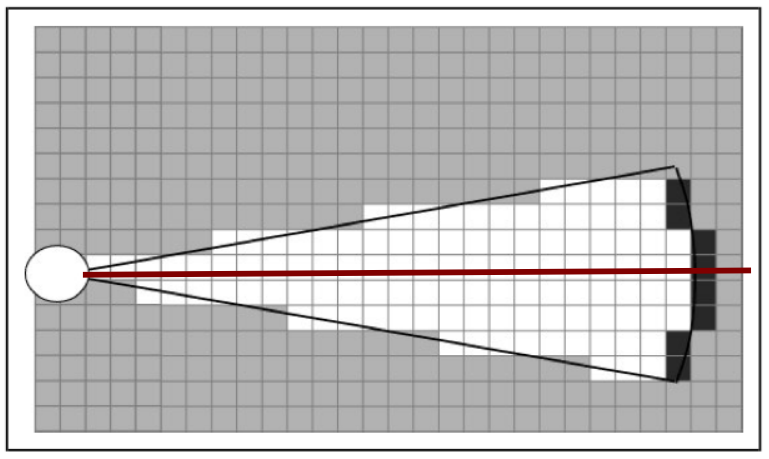
\includegraphics[width=0.7\textwidth]{figures/sonar_grid.png}
    \caption{Map grid cells in field of view of sonar sensor. Courtesy Burgard \cite{burgard_mr}.}
    \label{fig:sonar_grid}
\end{figure}

A few properties of the sensor is apparanet from Figure \ref{fig:sonar_grid}. Firstly, the sonar does not emit a directed beam in a specific direction, but has a deviation angle $\theta$ from which an emitted beam can be reflected back. Secondly, the sensor only detects the nearest object in its field of view (FOV), regardless of the view's width. This is can be shown by the arc of dark cells at the end of the beam, any of which can be the location of the real object. To deal with uncertainty in the measurement, a cell's modified probability depends on the cell's relative distance to the perceived obstacle and its deviation from the center of the sensor's orientation.

\begin{figure}
    \centering
    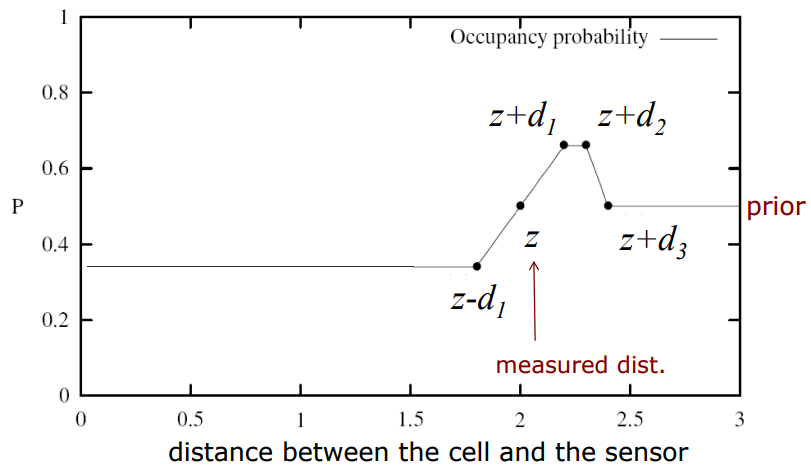
\includegraphics[width=0.8\textwidth]{figures/sonar_dist_p.png}
    \caption{Distance dependent probability update. Courtesy Burgard \cite{burgard_mr}.}
    \label{fig:sonar_dist_p}
\end{figure}

Figure \ref{fig:sonar_dist_p} describes the occupancy confidence of cells in the FOV, based on on where they are on the sensor distance line. The sensor confidence can be expressed in terms of constants $d_1, d_2, d_3$, which estimate the sensor noise and general thickness of obstacles. Cells that lay between $x_t$ and $z_t-d_1$ are perceived to be unoccupied, and will have a low probability, cells between $z_t-d_1$ and $z_t+d_1$ gradually increase in occupancy confidence as the measured distance approaches. Cells between $z_t+d_1$ and $z_t+d_2$ are regarded as obstructed, even with noise in the sensor it is reasonable to assume an obstruction $d_1$ further from the reading. Finally cells between $z_t+d_2$ and $z_t+d_3$ technically behind the sensed obstacle and thus no information about their occupancy is available. The same is true for cells beyond $z+d_3$. This can be evaluated in a piecewise function as

\begin{align}
    d &= \sqrt{(m_{i,x} - x_{t,x})^2 + (m_{i,y} - x_{t,y})^2} \\
    p(m_i) &= \left\{ \begin{array}{ll}
        p_{LOW} & d \leq z_t + d_1 \\
        p_{LOW} + \dfrac{p_{HIGH} - p_{LOW}}{2d_1} (d - z_t - d_1) & z_t-d_1 < d \leq z_t+d_1  \\
        p_{HIGH} & z_t+d_1 < d \leq z_t+d_2 \\
        p_{HIGH} - \dfrac{p_{HIGH} - p_0}{d_3 - d_2} (d - z_t+d_3) & z_t+d_2 < d \leq z_t+d_3 \\
        p_0 & d > z_t + d_3
    \end{array}
    \right.
\end{align}

\begin{figure}
    \centering
    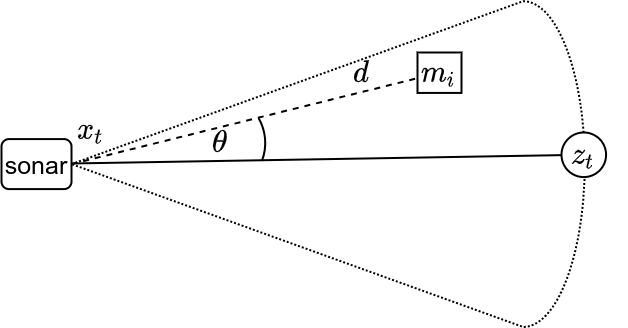
\includegraphics[width=0.7\textwidth]{figures/sonar_angle_p.png}
    \caption{Angle dependent probability update. Courtesy Burgard \cite{burgard_mr}.}
    \label{fig:sonar_angle_p}
\end{figure}

Figure \ref{fig:sonar_angle_p} shows a cell that is deviated from the center of the sonar's FOV by $\theta$. Assuming that sensor readings at a deviated angle will be less accurate and more prone to errors, it is wise to multiply the proposed confidence with a Gaussian distributed weight around the deviation $\theta$. The probability density function $f(x)$ of a normally distributed set equates to

\begin{align}
    f(x) &= \dfrac{1}{\sigma\sqrt{2\pi}} e^{-\dfrac{(x - \mu)^2}{2\sigma^2}}
\end{align}

with standard deviation $\sigma$ and mean $\mu = 0$, which can be used to calculate the Gaussian weight $s_\theta$ as

\begin{align}
    s_\theta &= \left\{ \begin{array}{ll}
        \dfrac{1}{\sigma\sqrt{2\pi}} e^{-\dfrac{\theta^2}{2\sigma^2}} & \theta \leq 0 \\
        \dfrac{1}{\sigma\sqrt{2\pi}} e^{-\dfrac{(1 - \theta)^2}{2\sigma^2}} & \theta > 0
    \end{array}
    \right.
\end{align}

Finally the measurement model can be expressed as

\begin{align}
    h(m_i, x_t, z_t) &= \log \dfrac{s_\theta p(m_i)}{1 - s_\theta p(m_i)}
\end{align}

Modern approaches tend to integrate the localization and mapping problems in one of several SLAM algorithms. This approach was not pursued intentionally as those algorithms require a lot of computational power and quite accurate distance readings. The proposed system has neither, working with a low-end microcontroller and low quality sonar sensors, but rather maps the world with known poses, thus it assumes localization is fairly accurate. The focus now shifts from a highly complex simultaneous optimization problem to ensuring accurate positioning, which is done through the incorporation of three different sensors in a sophisticated UKF for precise state estimation.

\subsubsection{Control}
\label{sec:control}

The passive aspects of the system have been dealt with, and the robot can effectively estimate its position and perceive the environment, but so far it is unable to plan paths nor act on those plans. In this section we assume a path has already been determined, and investigate the methods the robot employs to reach this goal accurately and timely.

The simplest control model aims to reach a desired state $x'$ from its current state $x$ by sending a set of controls $u$ to its actuators, producing state $y$. This model does not incorporate any perceptual information about the environment and is an open loop controller. This model is vastly insufficient for any system operating in the real world, as it does not account for noise, faulty actuators or dynamic unexpected events. A better model also incorporates sensor data to update the estimate of its state in what is known as a closed loop feedback controller.

\begin{figure}[H]
    \centering
    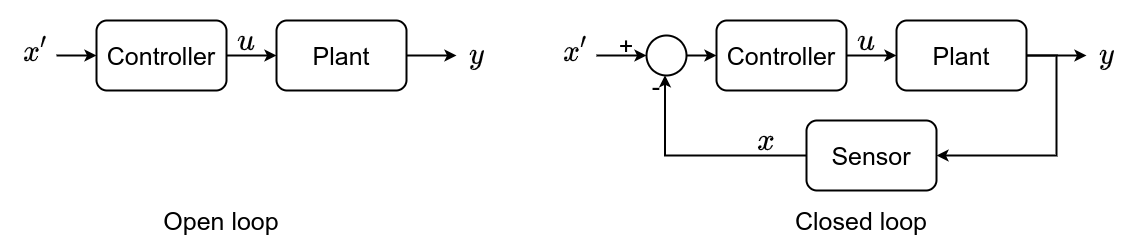
\includegraphics[width=\textwidth]{figures/open_loop.png}
    \caption{Open loop vs. closed loop controller}
    \label{fig:open_loop}
\end{figure}

A closed loop controller continually uses sensor data to update the error, $e$, between the desired and current states. The data flow model for a closed loop controller is given in Figure \ref{fig:closed_loop}, showing the interaction between the desired state $x_t'$, the current state $x_t$, the measured state $z_t$ and the input controls $u_t$. Process nosie $\epsilon_t$ and measurement noise $\delta_t$ also affect the system. The controller's objective is to relate the error between the desired and current state to the required input controls that will eventually result in the robot reaching the goal.

\begin{figure}[H]
    \centering
    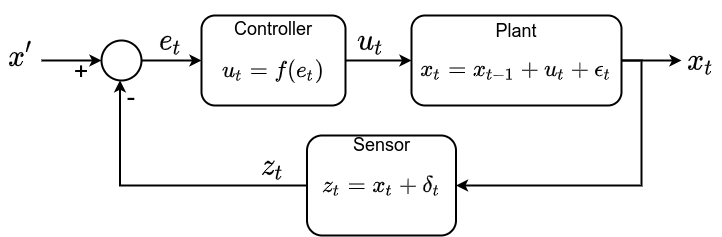
\includegraphics[width=0.8\textwidth]{figures/closed_loop.png}
    \caption{Closed loop controller data flow model}
    \label{fig:closed_loop}
\end{figure}

\textbf{PID controller theory}

Let us first examine a generic feedback controller with the above-mentioned parameters. The simplest controller would set the input proportional to the error,

\begin{align}
    u_t &= K_p (x' - x_t) \\
    &= K_p e_t, K_p < 1
    \label{eq:p-control}
\end{align}

where $K_p$ is the proportionality constant. Limiting $K_p$ to be less than one ensures that the system produces an input smaller than its perceived error, leading to a stable system response. On the other hand, if $K_p > 1$ the system would produce input larger than the error, which can lead to positive feedback and instability. 

The controller in Equation \ref{eq:p-control} works theoretically, but three physical phenomenon can degrade the quality of the system response. Firstly, the system is susceptible to noise, both in the actuators and in the sensors, which can lead to oscillations around the desired goal state, second a delay between the system's response and its perception of the reponse can lead to overcompensation for an action that has already been adjusted for, but due to inertia or sensor characteristics the effect is not seen yet. Thirdly, in the case where the system controls for the rate of change of a particular variable, such as the velocity of the robot's position, just reaching the desired position is not sufficient, as the system's velocity will cause it to overshoot. Rather the system should act in a manner to compensate for both its state and the rate of change of the state, to reach the goal state and remain there.

Noise and delay can be reduced by setting a lower value of $K_p$, but it can lead to a slower convergence rate. This is effectively a trade-off between fast convergence and low steady-state error, depending on the design requirements. In the latter case the system can be modelled more accurately according to Equation \ref{eq:pd-model}, accounting for both its state and its rate of change or derivative. This will ensure that the input is not only dependent on the magnitude of the error, but also the rate at which we are reducing the error, to ensure low oscillatory behaviour in the vicinity of the goal. As a bonus, the introduction of a derivative term facilitates the use of a larger stable proportional constant, leading to faster convergence.

\begin{align}
    x_t &= x_{t-1} + \Dot{x}\Delta t
    \label{eq:pd-model} \\
    u_t &= K_p (x' - x_t) + K_d (\Dot{x}' - \Dot{x}_t) \\
    u_t &= K_p e_t + K_d \dfrac{de_t}{dt}
\end{align}

A final modification can be made to the controller by considering the problem of steady state errors. These are small errors in the state when in the vicinity of the goal that accumulate over time to take the system off course. This is, for example, applicable if the desired state is a certain velocity to reach a faraway target, but due to a small deviation the target is not reached. Steady state errors are usually small enough that the proportional controller do not correct for them, or at least cannot do so effectively, as it is designed to deal with large inaccuracies. The solution is to correct for the integral of the error over time as part of the controller.

\begin{align}
    u_t &= K_p (x' - x_t) + K_d (\Dot{x}' - \Dot{x}_t) + K_i \int_0^t (x' - x_t) dt \\
    u_t &= K_p e_t + K_d \dfrac{de_t}{dt} + K_i \int_t e_t dt
\end{align}

The introduction of the integral term does however put the system in danger of the error build up, also known as the wind-up effect. If the robot does not act in the way it ought to, according to its model, which can happen if it is for example stuck in a hole. The integral error will continue to increase dramatically and completely disrupt the system once the robot comes out of the hole. The solution is to only integrate the error over fixed periods of time instead of over all possible time, which will at least contain the integral error to an upper manageable limit.

\textbf{Motor control}

With the theoretical foundation laid, we can proceed to the mathematical models of the motor and position controllers. The motor controller restricts its operation to the performance and expectation of the motors, and aims to reduce the error between the real and desired translational and rotational velocities $(v,\omega)$. This controller not only assumes that the desired position is known, but also that the position controller, described below, established the required velocities $(v,\omega)$ to reach the goal. The motivation for the separation of the two systems is that it produces a two modular, independent software components that can function semi-independent of one another, which eases development, debugging and maintenance. For the motor controller this allows a simplistic and focused model, and for the position controller this abstracts away the physical implementation of the velocities, once again simplifying and focusing its model.

The motor controller has state $\mathbf{x} = \{v, \omega\}$, where $v$ describes the forward velocity and $\omega$ the angular velocity of the robot. The desired state is of the same form $\mathbf{x}' = \{v', \omega'\}$. The input controls are the duty cycles that drive the PWM of the left and right motors, $\mathbf{u} = \{v_l, v_r\}$, and must have a value between -1 and 1. The sensors are the light-based odometers attached to the shafts of each wheel, which record the amount of holes $n$ in a wheel encoder that passes by in a specific time frame $\Delta t$. This is easily converted angular velocity of the wheel, $\omega_i$, and forward velocity, $v_i$, as

\begin{align}
    v_i &= r\omega_i = \dfrac{2 \pi r n}{N} \\
\end{align}

with $N$ the total amount of holes in the encoder and $r$ the radius of the wheels. The motor controller implements a simple proportional controller in as Equation \ref{eq:p-control-motor}.

\begin{align}
    \begin{bmatrix} v_r \\ v_l \end{bmatrix} &= K_p \begin{bmatrix}
        1 & K_\omega \\
        1 & -K_\omega
    \end{bmatrix} \begin{bmatrix}
        v' \\ \omega'
    \end{bmatrix}
    \label{eq:p-control-motor}
\end{align}

In essence the controller uses the translational velocity to set a velocity bar for both wheels, which is offset one way or another depending on the direction and magnitude of the desired angular velocity. 

\textbf{Position control}

The position controller aims to move the robot from its current position to its desired position by dynamically updating the required translational and angular velocities needed to get there. The controller has state $\mathbf{x} = \{x, y, \theta\}$, describing the current position and orientation of the robot in 2D state space, as well as desired state $\mathbf{x}'=\{x', y'\}$ as the goal and $\mathbf{u} = \{v, \omega\}$ as the input controls to the motor controller.

The first step is to obtain the distance and angular offset error between the current and desired state, which effectively converts the error to polar form.

\begin{align}
    e_t &= f(\mathbf{x}' - \mathbf{x}) \\
    \begin{bmatrix} e_r \\ e_\theta \end{bmatrix} &= \begin{bmatrix}
        \sqrt{(x' - x)^2 + (y' - y)^2} \\
        \text{atan2}(y' - y, x' - x) - \theta
    \end{bmatrix}
\end{align}

the C function \texttt{atan2()} is used as it respect the sign of the angle. Using the previous error states $e_{1:t-1}$, the integral and derivative terms can be calculated as

\begin{align}
    \int_0^t e_t d_t &= \sum_{i=0}^t e_i \Delta t = \sum_{i=0}^{t-1} e_i \Delta t + e_t \Delta t \\
    \dfrac{de_t}{dt} &= \dfrac{e_t - e_{t-1}}{\Delta t}
\end{align}

where the $\sum_{i=0}^{t-1} e_i \Delta t$ is the sum of all previous errors up to $e_{t-1}$ and is updated recursively. Finally the PID-controller can be implemented as

\begin{align}
    u_t &= K_p e_t + K_i \int_0^t e_t dt + K_d \dfrac{de_t}{dt} \\
    u_{t,v} &= K_{p,v} e_{t,r} + K_{i,v} \int_0^t e_{t,r} dt + K_{d,v} \dfrac{de_{t,r}}{dt} \\
    u_{t,\omega} &= K_{p,\omega} e_{t,\theta} + K_{i,\omega} \int_0^t e_{t,\theta} dt + K_{d,\omega} \dfrac{de_{t,\theta}}{dt}
\end{align}

There exists a inverse relationship between required velocity and estimated distance, thus to make sure velocity decreases with approaching speed, as well as to confine the suitable velocities to the hardware constraints of the system, the input controls are propagated through the following equation before being used in the motor control.

\begin{align}
	u_{t,v}' &= \dfrac{K_c u_{t,v}}{K_a + u_{t,v}}
\end{align}

where $K_c$ represents the hardware defined upper velocity limit, and $K_a$ is a modifier describing how the velocity should taper off as the robot approaches the goal position.

\subsubsection{Path planning}
\label{sec:path-plan}

\subsubsection{Navigation}
\label{sec:navigation}

\subsection{Simulations}
\label{sec:sim}

\subsection{Hardware Design and Implementation}

\subsubsection{Sensors}
\label{sec:sensors}

The autonomous vacuum cleaner has to interact with the environment in an intelligent manner, having knowledge of the landscape as well as its own observed actions. Thus, choosing the sensor components that will give real-time measurement input to the system is an integral first step in the journey towards robotic perception. The required input data aims to update the robot's perception of reality primarily in two ways: input that tells the robot about the environment, and input that observes the robot's actions. \\

The sensor input that describes the environment has to quantify the landscape by measuring the distance to obstacles in the horizontal plane close to the floor. Ideally the robot should be able to get a sense of the position of a measured obstacle relative to itself, thus both the distance to and the approximate direction of the obstacle is required. The potential sensor candidates include Lidar sensors, cameras, ultrasonic sensors and infrared scanners. \\

After thorough research and requirements evaluation it became clear that HC-SR04 ultrasonic sensors are the most suitable candidate for the system. An ultrasonic sensor is a distance sensing device that contains a transmitter and a receiver used to emit and receive an ultrasonic pulse respectively. Transmission of a 40kHz signal pattern starts while an echo pin is simultaneously pulled high until the transmitted pulse is reflected back into the receiver module. Measuring the length of the travelling pulse, while assuming that the speed of sound is known and approximately constant, the distance to the nearest obstacle in the direction of the sensor can easily be determined. The sensor does however have a $30^\circ$ total angular range or field of view within which the closest object will be detected. This leads to uncertainty in the exact location of the obstacle, as any position in a arc around the sensor's view could produce a reading at the specific distance. Despite this challenge, which will be addressed later on, the ultrasonic sensor is still the best sensor for the job due to the little post-processing required to interpret its measurement data, its large measurement range (2cm - 4m), its ability to operate in low lighting conditions and its relatively low power consumption, which is important for a system that runs on batteries. \\

\begin{figure}[H]
    \centering
    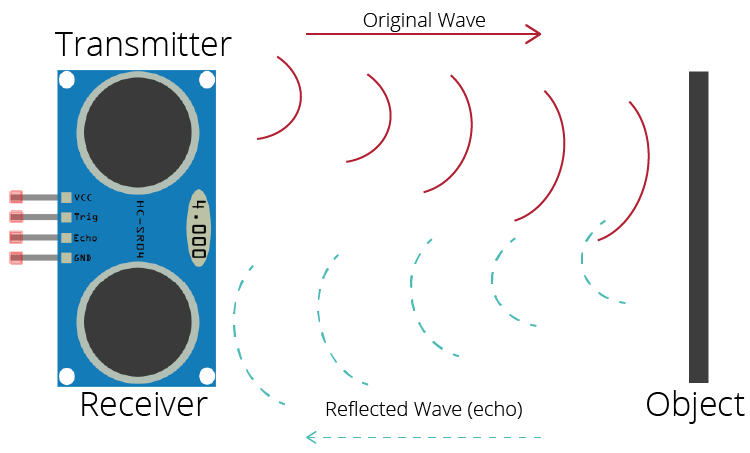
\includegraphics[width=0.5\textwidth]{figures/hcsr04_waves.png}
    \caption{HC-SR04 ultrasonic wave operation}
    \label{fig:hcsr04_waves}
\end{figure}

The system implements three HC-SR04 sensors in a semi-circle around the front of the robot, placed at such an angle that the three sensors collectively scan a $120^\circ$ field of view directly ahead of the robot, with each sensor placed offset by $40^\circ$ relative to one another. The $10^\circ$ blind spot produced by this design is small enough that it is highly unlikely that an obstruction can hide in there, without showing up in measurement readings on either side of the gap, especially across different samples taken at different locations. \\

A glaring limitation prohibits the use of higher resolution sensor components, such as cameras or lidar, which is the amount of processing power and more importantly, memory, required to effectively analyse incoming data. Computer vision algorithms are bulky and expensive, requiring tens of thousands of matrix operations and several levels of filtering, processing and AI-based sorting to work. These approaches are unfeasible for the simple, low-cost solution that this project aims to implement. Memory is a particularly constrained resource in an embedded system, with every single byte of stored space important. An array of photos in different processing stages taking up a few megabytes of storages is simply not an option. \\

The second set of sensors address the potential non-determinism in the robot's expected actions. The robot navigates the world by setting the duty cycle of the motors turning the wheels. This action is quite simple, but prone to process noise. For example, if both motors receive the same PWM duty cycle, the expected outcome is forward propagation in a straight line, but due to differences in friction, magnetic field strength and physical construction, one of the motors inevitable turns a little bit faster than the other one, which slowly takes the robot off course until it finds itself in a completely different location and orientation than its internal map of the world expects it to be. \\

The solution to actuator uncertainty involves an observation feedback loop coupled with a PI-controller, which will be explored in another section. The observation feedback loop observes properties of the robot that directly or indirectly provides information about the state of the device. These measurements are fused with the robots own estimation of its state to produce an updated state. Five sensor components are chosen for this task, a gyroscope, accelerometer and magnetometer combined in a 9-DOF IMU, as well as two odometers placed on the left and right wheels of the robot. Together these sensors can measure angular rate, velocity, acceleration and magnetic induction in three dimensions, potentially providing more than enough information to correct the robot's estimate of its state. \\

As the robot only operates on a 2D plane, assuming that the robot will never fall of a cliff (not that accurate positioning will be of much use in that case in anyway), we can neglect measurement data in certain dimensions, such as the roll and pitch of the gyroscope and the gravitational tug in the vertical direction from the accelerometer. This simplifies the sensor fusion algorithms as we focus on the sensor data that have a real impact on the positioning of the robot. \\

In summary, the gyroscope, accelerometer and magnetometer of the MPU9250 IMU sensor works in conjunction with two light emitting odometers attached to the wheels to accurate estimate the position of the robot in its internal map of the world. Unfortunately the accelerometer has to be placed on an exactly level plane to prohibit gravity from affecting the readings on the horizontal plane. The gyroscope is also infamous for large amounts of bias and bias instability, leading to wildly inaccurate readings. To overcome both of these problems, the robot stays in an initialization state for three seconds upon startup, during which at least 30 IMU sensor measurement are taken. As the robot is assumed to be stationary, any deviation from the expected values can be interpreted as bias. The average of the measured bias is subsequently subtracted from every measurement taken during navigation. This relaxes the requirement for a flat accelerometer and accurate gyroscope, and experimental results prove that this simple bias removal technic vastly improves the accuracy of the measurement model state estmation.

\subsubsection{Veroboard}
\label{sec:veroboard}

The veroboard design initially started out as a desperate attempt to build a working prototype after several iterations of PCB boards failed to work. As veroboards are a lot easier to change, redo and improve, a design choice was taken to stick to veroboard prototyping. The veroboard is home to a small ecosystem of components, each playing their part in making the system work as a whole. \\

The most important component on the board is the PIC32MX270F256-B microcontroller from Microchip, boasting a 40 MHz clock, 256kB of flash memory and 64kB of SRAM, as well as the MIPS32 RISC architecture. The chip has 28 pins, of which 17 can be used as general purpose input/output (GPIO) pins. With 14 peripheral devices, some requiring more than one pin, it seemed impossible to reconcile the large peripheral need with the low pin count. Fortunately, through a mixture of iteration, optimization and careful design, creative methods were developed to squeeze as much functionality out of the pins as possible. \\

For example, originally the three ultrasonic distance sensors each had to be triggered by a separate trigger pin to start a distance reading, while the measurement occured on another separate echo pin. Thus 6 out of 28 pins were wasted on one aspect of the peripheral components. Then it was discovered that the same echo pin can be reused if the correct assortment of diodes and resistors are used to pull the line low between readings and to eliminate power loss on the shared bus. So now we are down to three trigger pins and one echo pin. Triggering all three pins at once will result in potential crosstalk between the sensors and should be avoided. Finally it was found that triggering a pin and listening to an echo has the same characteristic pulse on a line, thus if the echo pin of sensor 1 is connected to the trigger pin of sensor 2, a completed measurement on sensor 1 will automatically start transmission on sensor 2. This was the final breakthrough that allowed the system to dedicate only 2 pins to all three ultrasonic sensors, while simplifying the code necessary to operate these components. \\

Another example is the sharing of the I$^2$C bus. The IMU, magnetometer and OLED display screen communicate via I$^2$C. Thus by connecting the three components to the same two wires can be used for SDA and SCL, using I$^2$C addressing to announce the recipient of a message. Lastly, further optimization took place by only dedicating one pin, TX to the UART, as it is assumed that the robot will not receive any data but will only be used to display information. \\

\subsubsection{Robot body}
\label{sec:robot} 

\subsubsection{Power management}
\label{sec:power}

Part of the design requirements of the robot describes the need to autonomously manage the robot's power consumption, whereby it returns back to the docking station (or starting location) once it detects low battery capacity. The robot can detect remaining capacity by measuring the voltage over the batteries. A single 18650 battery is fully charged at 4.2V, nominal at 3.7V and flat at 3.2V. The system has three 18650 batteries in series, thus it will be fully charged at 12.6V and dead at 9.6V. We would ideally want to halt operation and return back to the charger if the battery falls below 25\%, i.e. measured voltage is $<$ 10.2V. Of course, measuring voltages around 12V will completely fry a 3.3V chip, whereas simply lowering the voltage in a voltage divider will cause the applicable voltage range to be very small (2.5V - 3.3V). \\

Instead, the nature of electricity flow in the robot is used. The L298N H-bridge draws power from the batteries at their current varying voltage, but always outputs 5V to the veroboard circuit. By taking the scaled voltage difference between battery voltage and the 5V from the H-bridge in a differential amplifier, the complete range of the battery can be estimated more accurately.

\subsubsection{Vacuum pump}
\label{sec:vacuum}

\subsection{Software Design and Implementation}

\subsubsection{Peripheral drivers}
\label{sec:periph}

\subsubsection{Positioning and Sensor Fusion}
\label{sec:position}

\subsubsection{Mapping}
\label{sec:mapping}

\subsubsection{Motor Control}
\label{sec:control}

\subsubsection{Navigation}
\label{sec:navigation}



\subsubsection{Cleaning integration}
\label{sec:cleaning}

\subsection{Visual and statistical analysis}
\label{sec:stats}

\newpage

%% End of File.


%%
%%  Department of Electrical, Electronic and Computer Engineering.
%%  EPR400/2 Final Report - Section 4.
%%  Copyright (C) 2011-2021 University of Pretoria.
%%

\section{Results}

\subsection{Summary of results achieved}

\ldots

\subsection{Qualification tests}

\ldots

\newpage

%% End of File.



%%
%%  Department of Electrical, Electronic and Computer Engineering.
%%  EPR400/2 Final Report - Section 5.
%%  Copyright (C) 2011-2021 University of Pretoria.
%%

\section{Discussion}

\subsection{Interpretation of results}

\subsection{Critical evaluation of the design}

\subsection{Design ergonomics}

\subsection{Health, safety and environmental impact}

\subsection{Social and legal impact of the design}

\newpage

%% End of File.



%%
%%  Department of Electrical, Electronic and Computer Engineering.
%%  EPR400/2 Final Report - Section 6.
%%  Copyright (C) 2011-2021 University of Pretoria.
%%

\section{Conclusion}

\subsection{Summary of the work completed}

\subsection{Summary of the observations and findings}

\subsection{Contribution}

\subsection{Future work}

\newpage

%% End of File.




%% Use the IEEE Transactions style for the references.
\bibliographystyle{IEEEtran}
\bibliography{finalreport}
\newpage

%% --- PART 4 ------------------------------------------------------------

\eprsec{Part 4. Appendix: technical documentation}
\newpage

\setcounter{secnumdepth}{0}

\titleformat{\subsection}[display]
{\fontsize{14pt}{16.8pt}\selectfont\bfseries} {} {5pt} {\formatsubsectiontitle}
\titleformat{\subsection}[display]
{\fontsize{14pt}{16.8pt}\selectfont\bfseries} {} {5pt} {\formatsubsectiontitle}

%%
%%  Department of Electrical, Electronic and Computer Engineering.
%%  EPR400/2 Final Report - Technical Documentation.
%%  Copyright (C) 2011-2021 University of Pretoria.
%%

\section{HARDWARE part of the project}

\subsection{Record 1. System block diagram}


\subsection{Record 2.  Systems level description of the design}


\subsection{Record 3. Complete circuit diagrams and description}


\subsection{Record 4. Hardware acceptance test procedure}


\subsection{Record 5. User guide}


%% --------------------------------------------------------------------

\section{SOFTWARE part of the project}

\subsection{Record 6. Software process flow diagrams}


\subsection{Record 7. Explanation of software modules}


\subsection{Record 8. Complete source code}
Complete code has been submitted separately on the AMS.


\subsection{Record 9. Software acceptance test procedure}


\subsection{Record 10. Software user guide}


%% --------------------------------------------------------------------

\section{EXPERIMENTAL DATA}

\subsection{Record 11. Experimental data}


%% End of File.




\end{document}

%% End of File.
